%package list
\documentclass{article}
\usepackage[top=3cm, bottom=3cm, outer=3cm, inner=3cm]{geometry}
\usepackage{multicol}
\usepackage{graphicx}
\usepackage{url}
%\usepackage{cite}
\usepackage{hyperref}
\usepackage{array}
%\usepackage{multicol}
\newcolumntype{x}[1]{>{\centering\arraybackslash\hspace{0pt}}p{#1}}
\usepackage{natbib}
\usepackage{pdfpages}
\usepackage{multirow}    
\usepackage[normalem]{ulem}
\useunder{\uline}{\ul}{}
\usepackage{svg}
\usepackage{xcolor}
\usepackage{listings}
\lstdefinestyle{ascii-tree}{
    literate={├}{|}1 {─}{--}1 {└}{+}1 
  }

\lstset{basicstyle=\ttfamily,
  showstringspaces=false,
  commentstyle=\color{red},
  keywordstyle=\color{blue}
}
%\usepackage{booktabs}
\usepackage{caption}
\usepackage{subcaption}
\usepackage{float}
\usepackage{array}

\usepackage{enumitem}


\newcolumntype{M}[1]{>{\centering\arraybackslash}m{#1}}
\newcolumntype{N}{@{}m{0pt}@{}}


%%%%%%%%%%%%%%%%%%%%%%%%%%%%%%%%%%%%%%%%%%%%%%%%%%%%%%%%%%%%%%%%%%%%%%%%%%%%
%%%%%%%%%%%%%%%%%%%%%%%%%%%%%%%%%%%%%%%%%%%%%%%%%%%%%%%%%%%%%%%%%%%%%%%%%%%%
\newcommand{\itemEmail}{vmaldonadov@unsa.edu.pe}
\newcommand{\itemStudent}{Victor Gonzalo Maldonado Vilca}
\newcommand{\itemCourse}{Programación Web 2}
\newcommand{\itemCourseCode}{1702122}
\newcommand{\itemSemester}{III}
\newcommand{\itemUniversity}{Universidad Nacional de San Agustín de Arequipa}
\newcommand{\itemFaculty}{Facultad de Ingeniería de Producción y Servicios}
\newcommand{\itemDepartment}{Departamento Académico de Ingeniería de Sistemas e Informática}
\newcommand{\itemSchool}{Escuela Profesional de Ingeniería de Sistemas}
\newcommand{\itemAcademic}{2024 - A}
\newcommand{\itemInput}{Del 9 de abril de 2024}
\newcommand{\itemOutput}{Al 5 de junio de 2024}
\newcommand{\itemPracticeNumber}{07}
\newcommand{\itemTheme}{Django plantillas Destinos turísticos}
%%%%%%%%%%%%%%%%%%%%%%%%%%%%%%%%%%%%%%%%%%%%%%%%%%%%%%%%%%%%%%%%%%%%%%%%%%%%
%%%%%%%%%%%%%%%%%%%%%%%%%%%%%%%%%%%%%%%%%%%%%%%%%%%%%%%%%%%%%%%%%%%%%%%%%%%%

\usepackage[english,spanish]{babel}
\usepackage[utf8]{inputenc}
\AtBeginDocument{\selectlanguage{spanish}}
\renewcommand{\figurename}{Figura}
\renewcommand{\refname}{Referencias}
\renewcommand{\tablename}{Tabla} %esto no funciona cuando se usa babel
\AtBeginDocument{%
	\renewcommand\tablename{Tabla}
}

\usepackage{fancyhdr}
\pagestyle{fancy}
\fancyhf{}
\setlength{\headheight}{30pt}
\renewcommand{\headrulewidth}{1pt}
\renewcommand{\footrulewidth}{1pt}
\fancyhead[L]{\raisebox{-0.2\height}{
\includegraphics[width=3cm]{img/logo_episunsa.png}}}
\fancyhead[C]{\fontsize{7}{7}\selectfont	\itemUniversity \\ \itemFaculty \\ \itemDepartment \\ \itemSchool \\ \textbf{\itemCourse}}
\fancyhead[R]{\raisebox{-0.2\height}{
\includegraphics[width=1.2cm]{img/logo_abet}}}
\fancyfoot[L]{Victor M.}
\fancyfoot[C]{\itemCourse}
\fancyfoot[R]{Página \thepage}

% para el codigo fuente
\usepackage{listings}
\usepackage{color, colortbl}
\definecolor{dkgreen}{rgb}{0,0.6,0}
\definecolor{gray}{rgb}{0.5,0.5,0.5}
\definecolor{mauve}{rgb}{0.58,0,0.82}
\definecolor{codebackground}{rgb}{0.95, 0.95, 0.92}
\definecolor{tablebackground}{rgb}{0.8, 0, 0}

\lstset{frame=tb,
	language=bash,
	aboveskip=3mm,
	belowskip=3mm,
	showstringspaces=false,
	columns=flexible,
	basicstyle={\small\ttfamily},
	numbers=none,
	numberstyle=\tiny\color{gray},
	keywordstyle=\color{blue},
	commentstyle=\color{dkgreen},
	stringstyle=\color{mauve},
	breaklines=true,
	breakatwhitespace=true,
	tabsize=3,
	backgroundcolor= \color{codebackground},
}

\begin{document}
	
	\vspace*{10px}
	
	\begin{center}	
		\fontsize{17}{17} \textbf{ Informe de Laboratorio 07}
	\end{center}
	\centerline{\textbf{\Large Tema: \itemTheme}}
	%\vspace*{0.5cm}	

	\begin{flushright}
		\begin{tabular}{|M{2.5cm}|N|}
			\hline 
			\rowcolor{tablebackground}
			\color{white} \textbf{Nota}  \\
			\hline 
			     \\[30pt]
			\hline 			
		\end{tabular}
	\end{flushright}	

	\begin{table}[H]
		\begin{tabular}{|x{4.7cm}|x{4.8cm}|x{4.8cm}|}
			\hline 
			\rowcolor{tablebackground}
			\color{white} \textbf{Estudiante} & \color{white}\textbf{Escuela}  & \color{white}\textbf{Asignatura}   \\
			\hline 
			{\itemStudent \par \itemEmail} & \itemSchool & {\itemCourse \par Semestre: \itemSemester \par Código: \itemCourseCode}     \\
			\hline 			
		\end{tabular}
	\end{table}		
	
	\begin{table}[H]
		\begin{tabular}{|x{4.7cm}|x{4.8cm}|x{4.8cm}|}
			\hline 
			\rowcolor{tablebackground}
			\color{white}\textbf{Tarea} & \color{white}\textbf{Tema}  & \color{white}\textbf{Duración}   \\
			\hline 
			\itemPracticeNumber & \itemTheme & 2 horas   \\
			\hline 
		\end{tabular}
	\end{table}
	
	\begin{table}[H]
		\begin{tabular}{|x{4.7cm}|x{4.8cm}|x{4.8cm}|}
			\hline 
			\rowcolor{tablebackground}
			\color{white}\textbf{Semestre académico} & \color{white}\textbf{Fecha de inicio}  & \color{white}\textbf{Fecha de entrega}   \\
			\hline 
			\itemAcademic & \itemInput &  \itemOutput  \\
			\hline 
		\end{tabular}
	\end{table}
%%%%%%%%%%%%%%%%%%%%

  \section{Introducción}
  Django es un framework de desarrollo web en Python que facilita la creación rápida de aplicaciones web seguras y escalables.
  Ofrece un conjunto de herramientas integradas como ORM, administrador de Django y enrutamiento de URLs, lo que simplifica el 
  desarrollo y mejora la seguridad de las aplicaciones web.

%%%%%%%%%%%%%%%%%%%%

  \section{Objetivos}
  \begin{itemize}
    \item Implementar una aplicación en Django utilizando una plantilla profesional.
    \item Utilizar una tabla de Destinos turísticos para leer y completar la página web.
    \item Utilizar los tags “if” y “for” en los archivos html para leer todos los registros de una tabla desde una base de datos.
  \end{itemize}

%%%%%%%%%%%%%%%%%%%%
 
	\section{Tarea}
  \textbf{Ejercicios Propuestos}
  \begin{enumerate}
  \item Deberán replicar la actividad del video que se encuentra en el AV de Teoría (Django Tutorial for Beginners - Telusko https://youtu.be/OTmQOjsl0eg) donde se obtiene una plantilla de una aplicación de Destinos turísticos y adecuarla a un proyecto en blanco Django.
  \item Luego trabajar con un modelo de tabla DestinosTuristicos donde se guarden nombreCiudad,  descripcionCiudad, imagenCiudad, precioTour, ofertaTour (booleano).  Estos destinos turísticos deberán ser agregados en una vista dinámica utilizando tags for e if.
  \item Para ello crear una carpeta dentro del proyecto github colaborativo con el docente, e informar el link donde se encuentra.
  \item Crear formularios de Añadir Destinos Turísticos, Modificar, Listar y Eliminar Destinos.  
  \item Eres libre de agregar CSS para decorar tu trabajo.
  \item Ya sabes que el trabajo con Git es obligatorio.  Revisa el avance de la teoría Django parte4
  \end{enumerate}

 
%%%%%%%%%%%%%%%%%%%% 
 
  \section{Entregables}
  \begin{itemize}
    \item Informe hecho en Latex
    \item URL: Repositorio GitHub
    \item Link de Vídeo Explicativo (Youtube o flipgrid)
  \end{itemize}
  
%%%%%%%%%%%%%%%%%%%%    
		
	\section{Equipos, materiales y temas utilizados}
  \begin{itemize}
    \item Python
    \item Pip
    \item Django
    \item Entornos virtuales en python
    \item Proyectos de Django
    \item Aplicaciones en Django
    \item Modelos, Vistas, Templates y Formularios en Django
    \item Plantillas profesionales 
    \item Tags para vistas dinámicas

  \end{itemize}
 
%%%%%%%%%%%%%%%%%%%%

  \section{URL de Repositorio Github}
  \begin{itemize}
    \item URL del Repositorio GitHub
    \item \url{https://github.com/Victor-Gonzalo-Maldonado-Vilca/Lab07_Django.git}
  \end{itemize}
  
%%%%%%%%%%%%%%%%%%%%

	\section{Link de Video}
  \begin{itemize}
    \item Link del Vídeo Explicativo
    \item \textbf{Youtube: } \url{https://www.youtube.com/watch?v=pFaY1LSbvb8}
    \item \textbf{flipgrid: } \url{https://flip.com/s/jUuZm7UfskSd}
  \end{itemize}

%%%%%%%%%%%%%%%%%%%%

  \section{Metodología}

%%%%%%%%%%%%

  \subsection{Creación del entorno de Trabajo}
  
%%%%%%

  \subsubsection{Carpeta de trabajo}
  \begin{lstlisting}[language=, caption={Creación del Directorio}]
  mkdir lab07 && cd lab07
  \end{lstlisting}
  
%%%%%%

  \subsubsection{Creación del Entorno Virtual}
  \begin{lstlisting}[language=, caption={Creación Entorno virtual}]
  virtualenv -p python3 .
  \end{lstlisting}
  
%%%%%%%

  \subsubsection{Activar entorno Virtual}
  \begin{lstlisting}[language=, caption={Activar Entorno Virtual}]
  Scripts/activate
  \end{lstlisting}
  
%%%%%%

  \subsubsection{Instalar Django en el entorno Virtual}
  \begin{lstlisting}[language=, caption={Instalar Django}]
  pip install Django
  \end{lstlisting}
  
%%%%%%

  \subsubsection{Creación carpeta del proyecto}
  \begin{lstlisting}[language=, caption={Carpeta src}]
  mkdir src && cd src
  \end{lstlisting}
  
%%%%%%

  \subsubsection{Inicializar git}
  \begin{lstlisting}[language=, caption={Inicializar git}]
  git init
  \end{lstlisting}
  
%%%%%%

  \subsubsection{Crear .gitignore}
  Seguimos el siguiente Repositorio \url{https://github.com/django/django/blob/main/.gitignore}
  
%%%%%%%%%%%%
  
  \subsection{Creacion del proyecto y apps}
  
%%%%%%

  \subsubsection{Crear Proyecto}
  \begin{lstlisting}[language=, caption={Crear proyecto}]
  django-admin startproject telusko
  \end{lstlisting}
  
%%%%%%

  \subsubsection{Crear App}
  \begin{lstlisting}[language=, caption={Crear App}]
  python manage.py startapp travello
  \end{lstlisting}

%%%%%%%%%%%%%%%%%%%%

  \section{Desarrollo del trabajo}
  
%%%%%%%%%%%%

  \subsection{Seguimiento de la Actividad del Vídeo}
  \textit{Todo las app prueba se encuentran en el repositorio GitHub}
  \begin{itemize}
    \item Generación de proyectos Pruebas.
    \item El video nos otorga las plantillas, imágenes, js , css, etc para empezar con el proyecto.
    \item Link donde se encuentran los recursos: \url{https://www.dropbox.com/sh/gf8x8xjwidq20cz/AABPlOsXmijnz0-yjxYj9ebsa?dl=0}
    \begin{figure}[H]
      \centering
      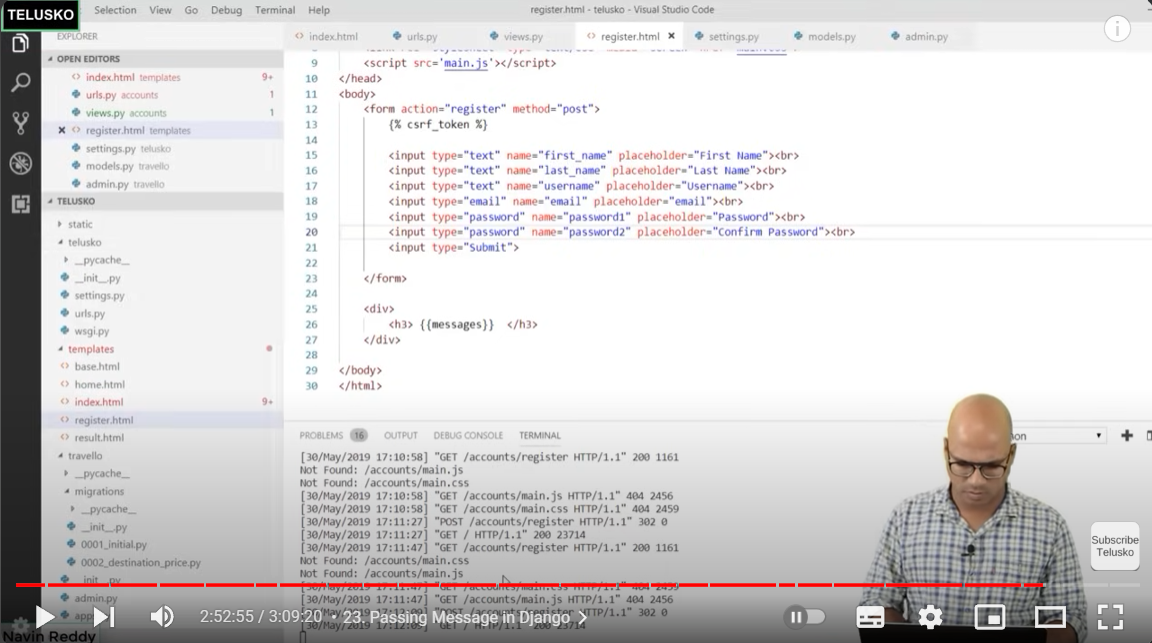
\includegraphics[width=1\textwidth, keepaspectratio]{img/video.png}
      \caption{Imágen del vídeo}
    \end{figure}
    \newpage
  \end{itemize}
  
%%%%%%%%%%%%

  \subsection{Configuración en settings.py}
  
%%%%%%

  \subsubsection{Configuración del Lenguaje y Time-Zone}
  \begin{figure}[H]
    \centering
    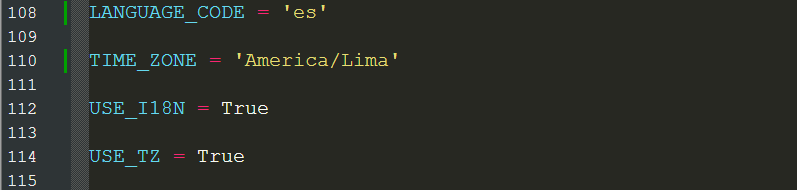
\includegraphics[width=1\textwidth, keepaspectratio]{img/lenguaje.png}
    \caption{Internationalization}
  \end{figure}
  
%%%%%%

  \subsubsection{Configuración de archivos estáticos}
  \begin{figure}[H]
    \centering
    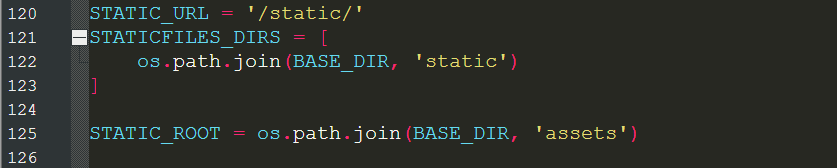
\includegraphics[width=1\textwidth, keepaspectratio]{img/static.png}
    \caption{Static Files}
  \end{figure}
  
%%%%%%

  \subsubsection{Configuración de archivos media}
  \begin{figure}[H]
    \centering
    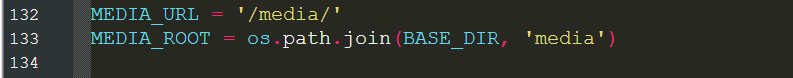
\includegraphics[width=1\textwidth, keepaspectratio]{img/media.png}
    \caption{Media Files}
  \end{figure}
  
%%%%%%%%%%%%

  \subsection{Modelos}
  
%%%%%%

  \subsubsection{Modelo tabla DiseñoTuristico}
  \begin{itemize}
    \item \textbf{Descripción: }El modelo Destination representa destinos turísticos e incluye campos como el nombre de la ciudad 
    (nombreCiudad), una descripción detallada de la ciudad (descripcionCiudad), una imagen representativa de la ciudad (imagenCiudad), 
    el precio del tour (precioTour), y un indicador de si hay una oferta de tour disponible (ofertaTour).
    \begin{lstlisting}[language=Python, caption={Modelo Destination}]
    class Destination(models.Model):
      nombreCiudad = models.CharField(max_length=100)
      descripcionCiudad = models.TextField()
      imagenCiudad = models.ImageField(upload_to='images/', default='default_image.jpg')
      precioTour = models.DecimalField(max_digits=10, decimal_places=2)
      ofertaTour = models.BooleanField(default=False)

      def __str__(self):
          return self.nombreCiudad
    \end{lstlisting}
  \end{itemize}
  
%%%%%%

  \subsubsection{Modelo Para Eliminar Lugares Turísticos}
  \begin{itemize}
    \item \textbf{Descripción: }El modelo Delete esta relacionado con la eliminación de ciudades, ya que solo tiene un campo para el 
    nombre de la ciudad (nombreCiudad).
    \begin{lstlisting}[language=Python, caption={Modelo Delete}]
    class Delete(models.Model):
      nombreCiudad = models.CharField(max_length=100)
      
      def __str__(self):
          return self.nombreCiudad
    \end{lstlisting}
  \end{itemize}
  
%%%%%%

  \subsubsection{Modelo Para Modificar Lugares Turísticos}
  \begin{itemize}
    \item \textbf{Descripción: }El modelo Modificar tiene un campo para el nombre de la ciudad (nombreCiudad), despues se enviara como argumento
     este campo a otra página web donde se podra realizar cambios al Lugar Turístico seleccionado.
    \begin{lstlisting}[language=Python, caption={Modelo Modificar}]
    class Modificar(models.Model):
      nombreCiudad = models.CharField(max_length=100)
      
      def __str__(self):
          return self.nombreCiudad
    \end{lstlisting}
  \end{itemize}
  
%%%%%%%%%%%%

  \subsection{Creación de los Formularios Añadir, Modificar, Listar y Eliminar}
  
%%%%%%

  \subsubsection{Formulario DestinationForm - Análogo de Añadir}
  \begin{itemize}
    \item \textbf{Descripción: }El formulario DestinationForm está asociado con el modelo Destination y contiene campos para 
    ingresar información como el nombre de la ciudad, su descripción, una imagen representativa, el precio del tour y la disponibilidad de ofertas.
    \begin{lstlisting}[language=Python, caption={Formulario Añadir}]
    class DestinationForm(forms.ModelForm):
      class Meta:
          model = Destination
          fields = ['nombreCiudad', 'descripcionCiudad', 'imagenCiudad', 'precioTour', 'ofertaTour']
    \end{lstlisting}
  \end{itemize}
  \newpage
  
%%%%%%

  \subsubsection{Formulario ModificarForm - Análogo de Modificar}
  \begin{itemize}
    \item \textbf{Descripción: }El formulario ModificarForm corresponde al modelo Modificar y tiene un campo para ingresar el 
    nombre de la ciudad que se desea modificar.
    \begin{lstlisting}[language=Python, caption={Formulario Modificar}]
    class ModificarForm(forms.ModelForm):
      class Meta:
          model = Modificar
          fields = ['nombreCiudad']
    \end{lstlisting}
  \end{itemize}
  
%%%%%%

  \subsubsection{Formulario ModificarFormu - Análogo de Modificar}
  \begin{itemize}
    \item \textbf{Descripción: }El formulario ModificarFormu es una variante del DestinationForm pero con otro propósito, este logrará que los datos
     se actualicen.
    \begin{lstlisting}[language=Python, caption={Formulario Modificar}]
    class ModificarFormu(forms.ModelForm):
      class Meta:
          model = Destination
          fields = ['nombreCiudad', 'descripcionCiudad', 'imagenCiudad', 'precioTour', 'ofertaTour']
    \end{lstlisting}
  \end{itemize}
  
%%%%%%

  \subsubsection{Formulario DeleteForm - Análogo de Eliminar}
  \begin{itemize}
    \item \textbf{Descripción: }El formulario DeleteForm está vinculado al modelo Delete y proporciona un campo para ingresar 
    el nombre de la ciudad que se desea eliminar.
    \begin{lstlisting}[language=Python, caption={Formulario Eliminar}]
    class DeleteForm(forms.ModelForm):
      class Meta:
          model = Delete
          fields = ['nombreCiudad']
    \end{lstlisting}
  \end{itemize}
  
%%%%%%

  \subsubsection{Formulario Listar}
  \begin{itemize}
    \item \textbf{Descripción: }No se requiere formularios para esta sección, solo tags for e if.
  \end{itemize}
  
%%%%%%%%%%%%

  \subsection{Vistas}
  
%%%%%%

  \subsubsection{Vista index}
  \begin{itemize}
    \item \textbf{Descripción: }La vista index recupera todos los destinos de la base de datos utilizando el modelo Destination 
    y los pasa al template index.html como parte del contexto para renderizar la página principal.
    \begin{lstlisting}[language=Python, caption={index}]
    def index(request):
      destinos = Destination.objects.all()
      context = {'destinos': destinos}
      return render(request, 'index.html', context)
    \end{lstlisting}
  \end{itemize}
  \newpage
  
%%%%%%

  \subsubsection{Vistas about, contact y news}
  \begin{itemize}
    \item \textbf{Descripción: }Las vistas about, contact y news simplemente renderizan las páginas correspondientes (about.html, contact.html y news.html) 
    sin realizar ninguna operación adicional.
    \begin{lstlisting}[language=Python, caption={about}]
    def about(request):
      return render(request, 'about.html');
    \end{lstlisting}
    \begin{lstlisting}[language=Python, caption={contact}]
    def contact(request):
      return render(request, 'contact.html');
    \end{lstlisting}
    \begin{lstlisting}[language=Python, caption={news}]
    def news(request):
      return render(request, 'news.html');
    \end{lstlisting}
  \end{itemize}
  
%%%%%%

  \subsubsection{Vista admin}
  \begin{itemize}
    \item \textbf{Descripción: }La vista admin maneja la lógica para la administración de destinos. Crea instancias 
    de formularios para crear, eliminar y modificar destinos, recupera todos los destinos de la base de datos y procesa 
    las solicitudes POST según la acción realizada por el usuario (crear, eliminar o modificar).
    \begin{lstlisting}[language=Python, caption={admin}]
    def admin(request):
      crear_form = DestinationForm()
      eliminar_form = DeleteForm()
      modificar_form = ModificarForm()
      destinos = Destination.objects.all()
      
      if request.method == 'POST':
          if 'crear' in request.POST:
              crear_form = DestinationForm(request.POST, request.FILES)
              if crear_form.is_valid():
                  crear_form.save()
                  return redirect('admin')
          elif 'eliminar' in request.POST:
              eliminar_form = DeleteForm(request.POST)
              if eliminar_form.is_valid():
                  nombre_ciudad = eliminar_form.cleaned_data['nombreCiudad']
                  destino = get_object_or_404(Destination, nombreCiudad=nombre_ciudad)
                  destino.delete()
                  return redirect('admin')
          elif 'modificar' in request.POST:
              nombre_ciudad = request.POST.get('nombreCiudad')
              try:
                  lugar = Destination.objects.get(nombreCiudad=nombre_ciudad)
                  return redirect('modificar', ciudad=nombre_ciudad)
              except Destination.DoesNotExist:
                  return redirect('admin')
              
      
      context = {
          'crear_form': crear_form,
          'eliminar_form': eliminar_form,
          'modificar_form': modificar_form,
          'destinos': destinos,
      }
      return render(request, 'admin.html', context)
    \end{lstlisting}
  \end{itemize}
  
%%%%%%

  \subsubsection{Vista modificar}
  \begin{itemize}
    \item \textbf{Descripción: }La vista modificar maneja la lógica para modificar un destino específico. 
    Recupera el destino a modificar utilizando su nombre de ciudad, crea un formulario prellenado con los datos existentes 
    del destino y guarda los cambios realizados por el usuario si el formulario es válido.
    \begin{lstlisting}[language=Python, caption={modificar}]
    def modificar(request, ciudad):
      lugar = get_object_or_404(Destination, nombreCiudad=ciudad)
      form = ModificarFormu(instance=lugar)
      
      if request.method == 'POST':
          form = ModificarFormu(request.POST, instance=lugar)
          if form.is_valid():
              form.save()
              return redirect('admin')
      
      context = {
          'form': form,
      }
      return render(request, 'modificar.html', context)
    \end{lstlisting}
  \end{itemize}

%%%%%%%%%%%%

  \subsection{URLs}
  
%%%%%%

  \subsubsection{urls.py del proyecto telusko}
  \begin{itemize}
    \item \textbf{Descripción: }Este bloque de código configura las URL para el proyecto Django telusko, asignando las URL 
    a vistas específicas y proporcionando la capacidad de servir archivos estáticos y de medios en modo DEBUG.
    \begin{lstlisting}[language=Python, caption={urls Telusko}]
    urlpatterns = [
      path('travello', include('travello.urls')),  
      path('admin/', admin.site.urls),
    ]

    if settings.DEBUG:
      urlpatterns += static(settings.MEDIA_URL, document_root=settings.MEDIA_ROOT)
    \end{lstlisting}
  \end{itemize}
  
%%%%%%

  \subsubsection{urls.py de la app travello}
  \begin{itemize}
    \item \textbf{Descripción: }Este bloque de código definen las rutas accesibles en el sitio web y las asocian con las vistas 
    correspondientes para manejar las solicitudes de los usuarios.
    \begin{lstlisting}[language=Python, caption={urls Travello}]
    urlpatterns = [
      path('',views.index, name='index'),
      path('about/', views.about, name='about'),
      path('contact/',views.contact, name='contact'),
      path('news/',views.news, name='news'),
      path('admin/',views.admin, name='admin'),
      path('/modificar/<str:ciudad>/', views.modificar, name='modificar'),
    ]
    \end{lstlisting}
  \end{itemize}
  
%%%%%%%%%%%%

  \subsection{Plantillas}
  \textit{Las plantillas que se omitiran serán las presentadas en el vídeo que se debio seguir, se centrar en la plantilla admin y modificar. 
  Recordemos que las plantillas deben estar en la carpeta templates}
  
%%%%%%

  \subsubsection{Plantilla admin.html}
  \begin{itemize}
    \item \textbf{Descripción: }Esta línea carga los archivos estáticos (como CSS, JavaScript) para que puedan ser utilizados en la página.
    \begin{lstlisting}[language=html]
    
    \end{lstlisting}
    \item \textbf{Descripción: }Define la estructura básica del documento HTML, incluyendo el título de la página y el enlace al archivo 
    CSS para estilos.
    \begin{lstlisting}[language=html]
    <head>
      <title>Administrar Lugares</title>
      <link rel="stylesheet" type="text/css" href="">
    </head>
    \end{lstlisting}
    \item \textbf{Descripción: }Formulario para agregar un nuevo lugar, con un campo para cada atributo del modelo Destination y un 
    botón para guardar los datos. 
    \begin{lstlisting}[language=html]
    <h1>Agregar Lugar</h1>
    <form method="post" enctype="multipart/form-data">
      
      {{ crear_form.as_p }}
      <button type="submit" name="crear">Guardar</button>
    </form>
    \end{lstlisting}
    \newpage
    \item \textbf{Descripción: }Formulario para eliminar un lugar existente, con un campo para seleccionar el nombre de la ciudad y un 
    botón para eliminar el lugar.
    \begin{lstlisting}[language=html]
    <h1>Eliminar Lugar</h1>
    <form method="post">
      
      {{ eliminar_form.as_p }}
      <button type="submit" name="eliminar">Guardar</button>
    </form>
    \end{lstlisting}
    \item \textbf{Descripción: }Formulario para modificar un lugar existente, con un campo para seleccionar el nombre de la ciudad y 
    un botón para redireccionar a modificar.html pasando como argumento la ciudad.
    \begin{lstlisting}[language=html]
    <h1>Modificar Lugar</h1>
    <form method="post">
      
      {{ modificar_form.as_p }}
      <button type="submit" name="modificar">Guardar</button>
    </form>
    \end{lstlisting}
    \item \textbf{Descripción: }Sección para mostrar los lugares existentes, incluyendo imágenes, nombres, descripciones, precios y ofertas.
    \begin{lstlisting}[language=html]
    
      <div class="row">
        <div class="col">
          
          <div class="destination item">
            <div class="destination_image">
              <img src="{{ destino.imagenCiudad.url }}" alt="{{ destino.nombreCiudad }} Image">
            </div>
            <div class="destination_content">
              <div class="destination_title">{{ destino.nombreCiudad }}</div>
              <div class="destination_subtitle"><p>{{ destino.descripcionCiudad }}</p></div>
              <div class="destination_price">$ {{ destino.precioTour }} - Oferta: {{ destino.ofertaTour }}</div>
            </div>
          </div>
          
        </div>
      </div>
    
    \end{lstlisting}
    \item \textbf{Descripción: }Enlace para regresar a la página principal (index.html) del sitio web.
    \begin{lstlisting}[language=html]
    <div class="main-link">
      <a href="">Pagina Principal</a>
    </div>
    \end{lstlisting}
  \end{itemize}
  \newpage
  
%%%%%%

  \subsubsection{Plantilla modificar.html}
  \begin{itemize}
    \item \textbf{Descripción: }Esta línea carga los archivos estáticos (como CSS, JavaScript) para que puedan ser utilizados en la página.
    \begin{lstlisting}[language=html]
    
    \end{lstlisting}
    \item \textbf{Descripción: }Define la estructura básica del documento HTML, incluyendo el título de la página y el enlace al archivo 
    CSS para estilos.
    \begin{lstlisting}[language=html]
    <head>
      <title>Modificar Lugar</title>
      <link rel="stylesheet" type="text/css" href="">
    </head>
    \end{lstlisting}
    \item \textbf{Descripción: }Formulario para modificar un lugar existente. Incluye un campo para cada atributo del modelo asociado al formulario y 
    un botón para guardar los cambios.
    \begin{lstlisting}[language=html]
    <h1>Modificar Lugar</h1>
    <form method="post" enctype="multipart/form-data">
      
      {{ form.as_p }}
       <button type="submit" name="crear">Guardar</button>
    </form>
    \end{lstlisting}
  \end{itemize}
  
%%%%%%%%%%%%

  \subsection{Estilos}
  \textit{Los estilos fueron entregados por el vídeo seguido, además los estilos de las anteriores plantillas solo son cambio de color, estos se encuentran en el repositorio GitHub}
  
%%%%%%

  \subsubsection{Styles de admin.html}
  \begin{lstlisting}[language=]
  body {
    font-family: Arial, sans-serif;
    margin: 0;
    padding: 0;
    background-color: #f4f4f4;
  }

  h1 {
    color: #333;
    text-align: center;
    padding: 20px;
  }

  form {
    width: 50%;
    margin: 0 auto;
    padding: 20px;
    background-color: #fff;
    border-radius: 8px;
    box-shadow: 0 0 10px rgba(0, 0, 0, 0.1);
  }

  form button {
    display: block;
    width: 100%;
    padding: 10px;
    background-color: #5cb85c;
    color: #fff;
    border: none;
    border-radius: 5px;
    cursor: pointer;
    font-size: 16px;
  }

  form button:hover {
    background-color: #4cae4c;
  }

  .destinations {
    padding: 20px;
  }

  .destination {
    background-color: #fff;
    border-radius: 8px;
    margin-bottom: 20px;
    overflow: hidden;
    box-shadow: 0 0 10px rgba(0, 0, 0, 0.1);
    text-align: center;
  }

  .destination_image img {
    width: 25%;
    height: auto;
    display: block;
    margin-left: auto;
    margin-right: auto;
  }

  .destination_content {
    padding: 20px;
    text-align: center;
  }

  .destination_title {
    font-size: 20px;
    font-weight: bold;
    color: #333;
  }

  .destination_subtitle {
    font-size: 14px;
    color: #777;
    margin-top: 10px;
  }

  .destination_price {
    font-size: 18px;
    color: #e67e22;
    margin-top: 10px;
  }

  .container {
    max-width: 1200px;
    margin: 0 auto;
  }

  .section_title {
    font-size: 28px;
    margin-top: 20px;
  }

  .main-link {
    text-align: center;
    margin: 20px;
  }

  .main-link a {
    color: #337ab7;
    font-size: 18px;
    text-decoration: none;
    padding: 10px 20px;
    border: 1px solid #337ab7;
    border-radius: 5px;
    transition: background-color 0.3s, color 0.3s;
  }

  .main-link a:hover {
    background-color: #337ab7;
    color: #fff;
  }
  \end{lstlisting}
  
%%%%%%

  \subsubsection{Styles de modificar.html}
  \begin{lstlisting}[language=]
  body {
    font-family: Arial, sans-serif;
    margin: 0;
    padding: 0;
    background-color: #f4f4f4;
  }

  h1 {
      color: #333;
      text-align: center;
      padding: 20px;
  }

  form {
      width: 50%;
      margin: 0 auto;
      padding: 20px;
      background-color: #fff;
      border-radius: 8px;
      box-shadow: 0 0 10px rgba(0, 0, 0, 0.1);
  }

  form button {
      display: block;
      width: 100%;
      padding: 10px;
      background-color: #5cb85c;
      color: #fff;
      border: none;
      border-radius: 5px;
      cursor: pointer;
      font-size: 16px;
  }

  form button:hover {
      background-color: #4cae4c;
  }

  \end{lstlisting}
  
%%%%%%%%%%%%

  \subsection{Ejecución}
  \textit{Usamos "python manage.py runserver"}
  \begin{figure}[H]
    \centering
    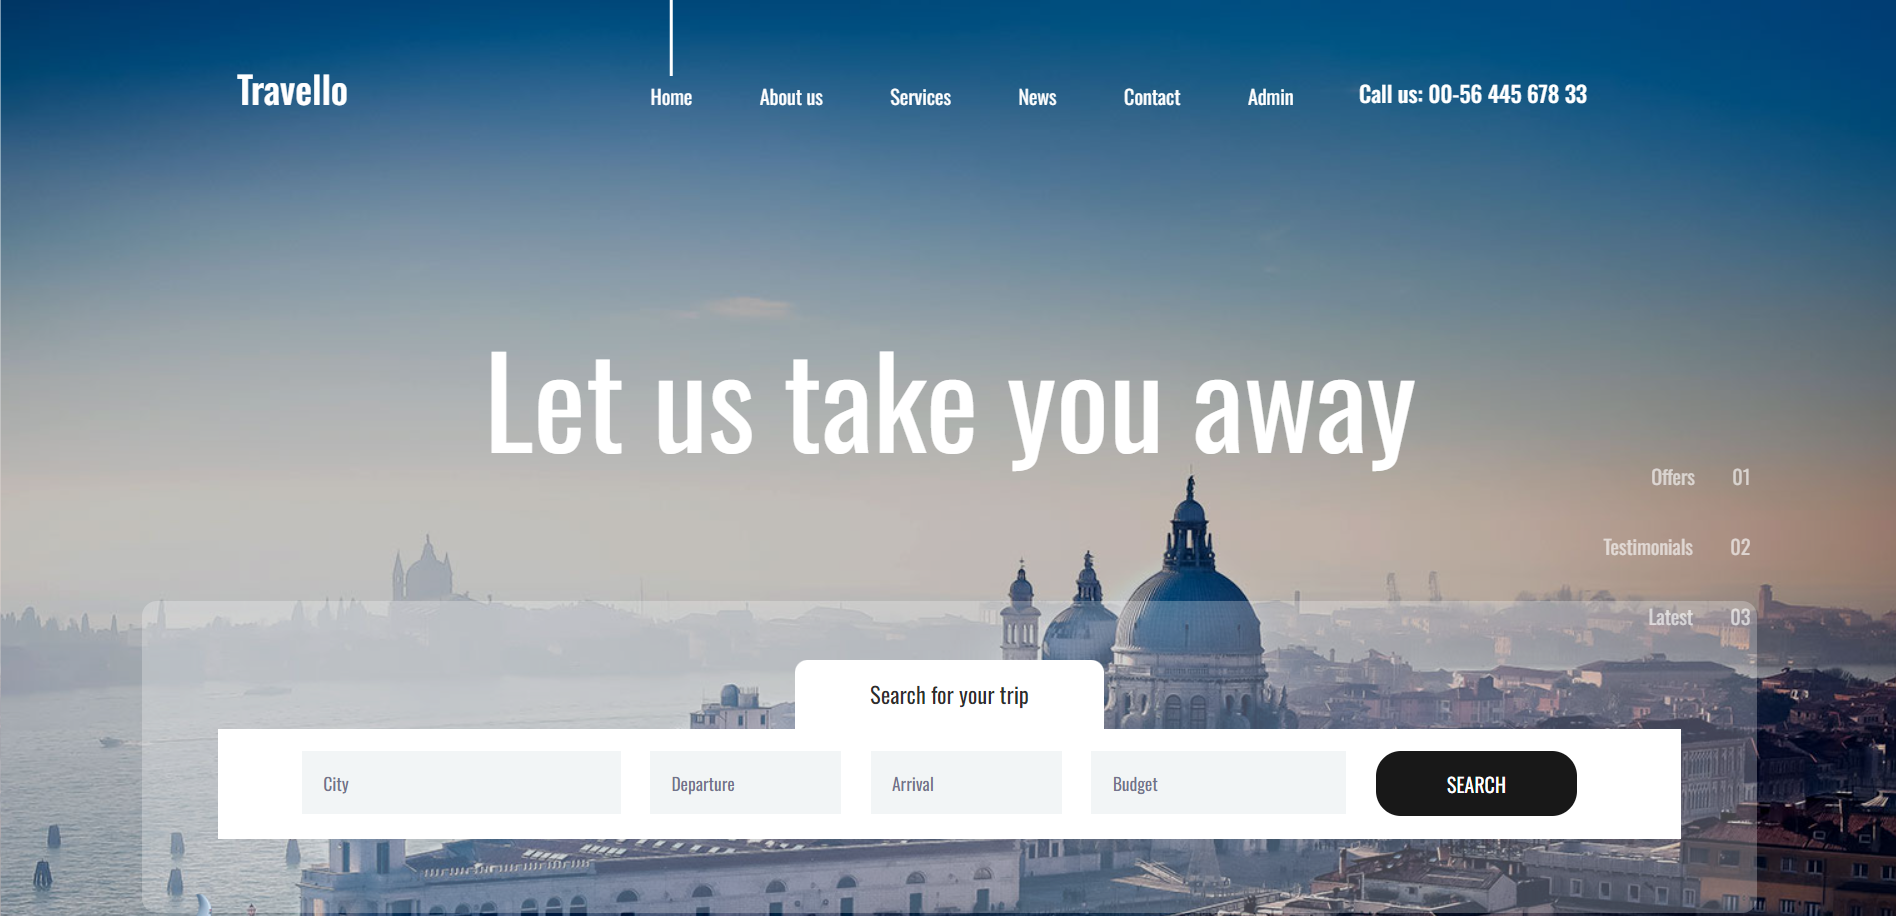
\includegraphics[width=1\textwidth, keepaspectratio]{img/ejecucion1.png}
    \caption{Home}
  \end{figure}
  \newpage
  \begin{figure}[H]
    \centering
    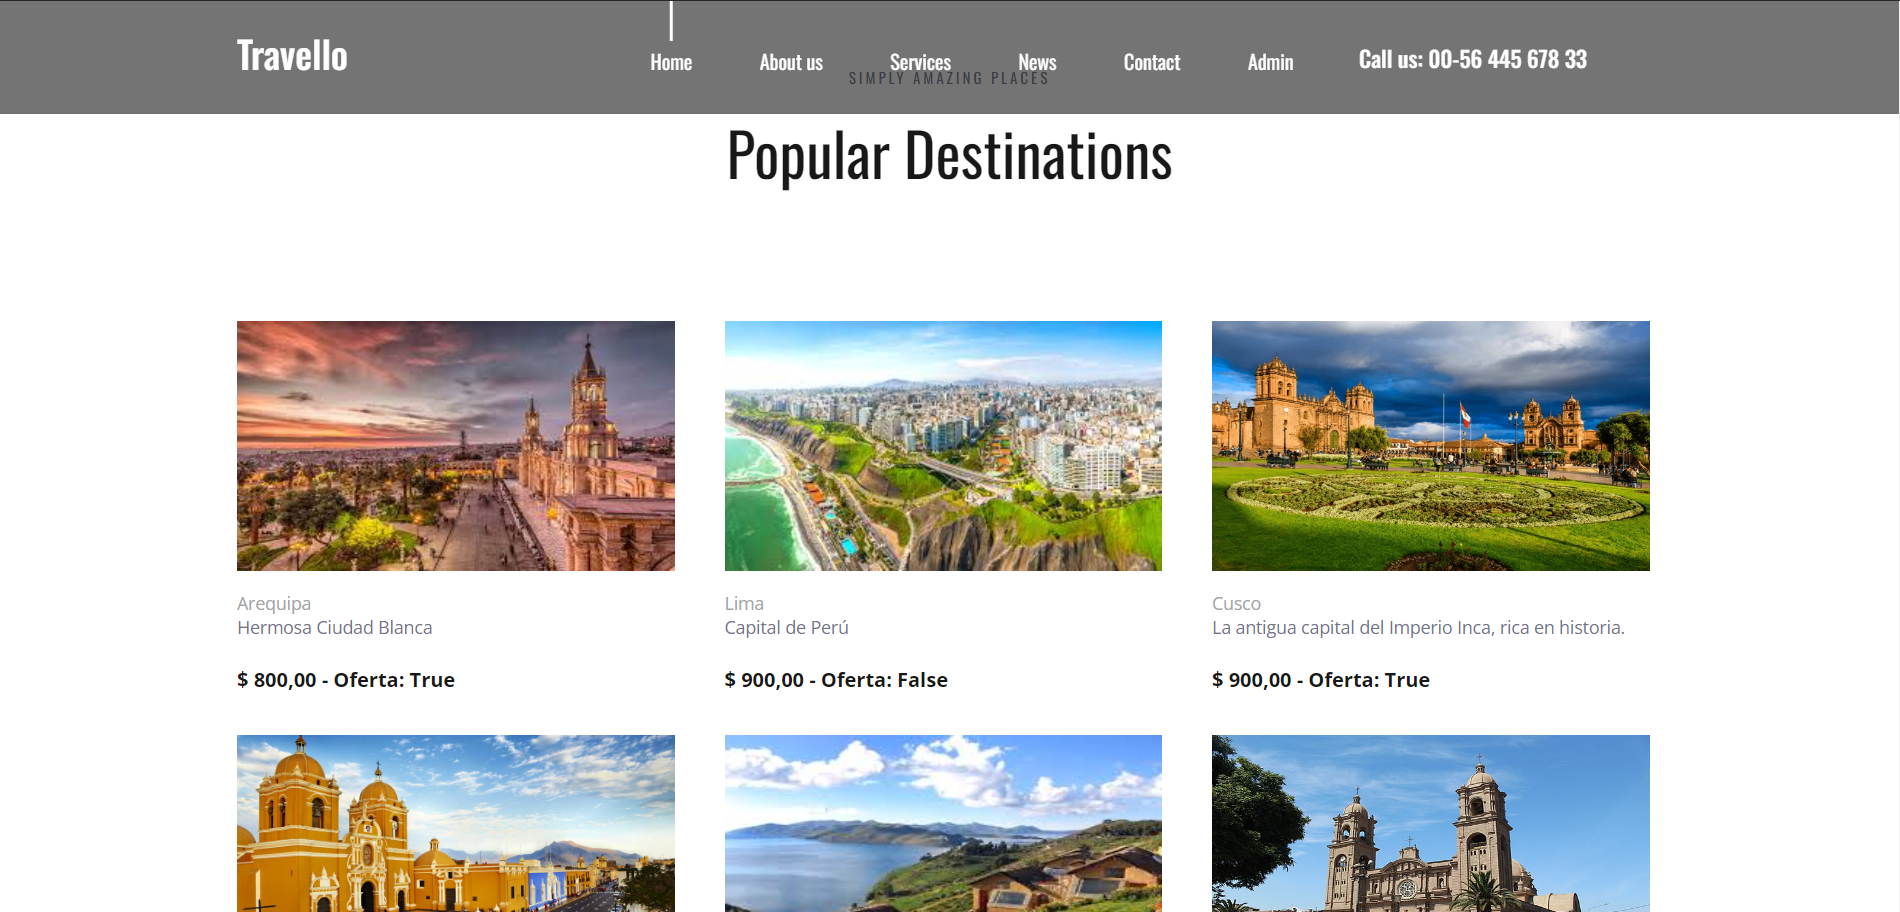
\includegraphics[width=1\textwidth, keepaspectratio]{img/ejecucion2.png}
    \caption{Listar con tag for e if}
  \end{figure}
  \begin{figure}[H]
    \centering
    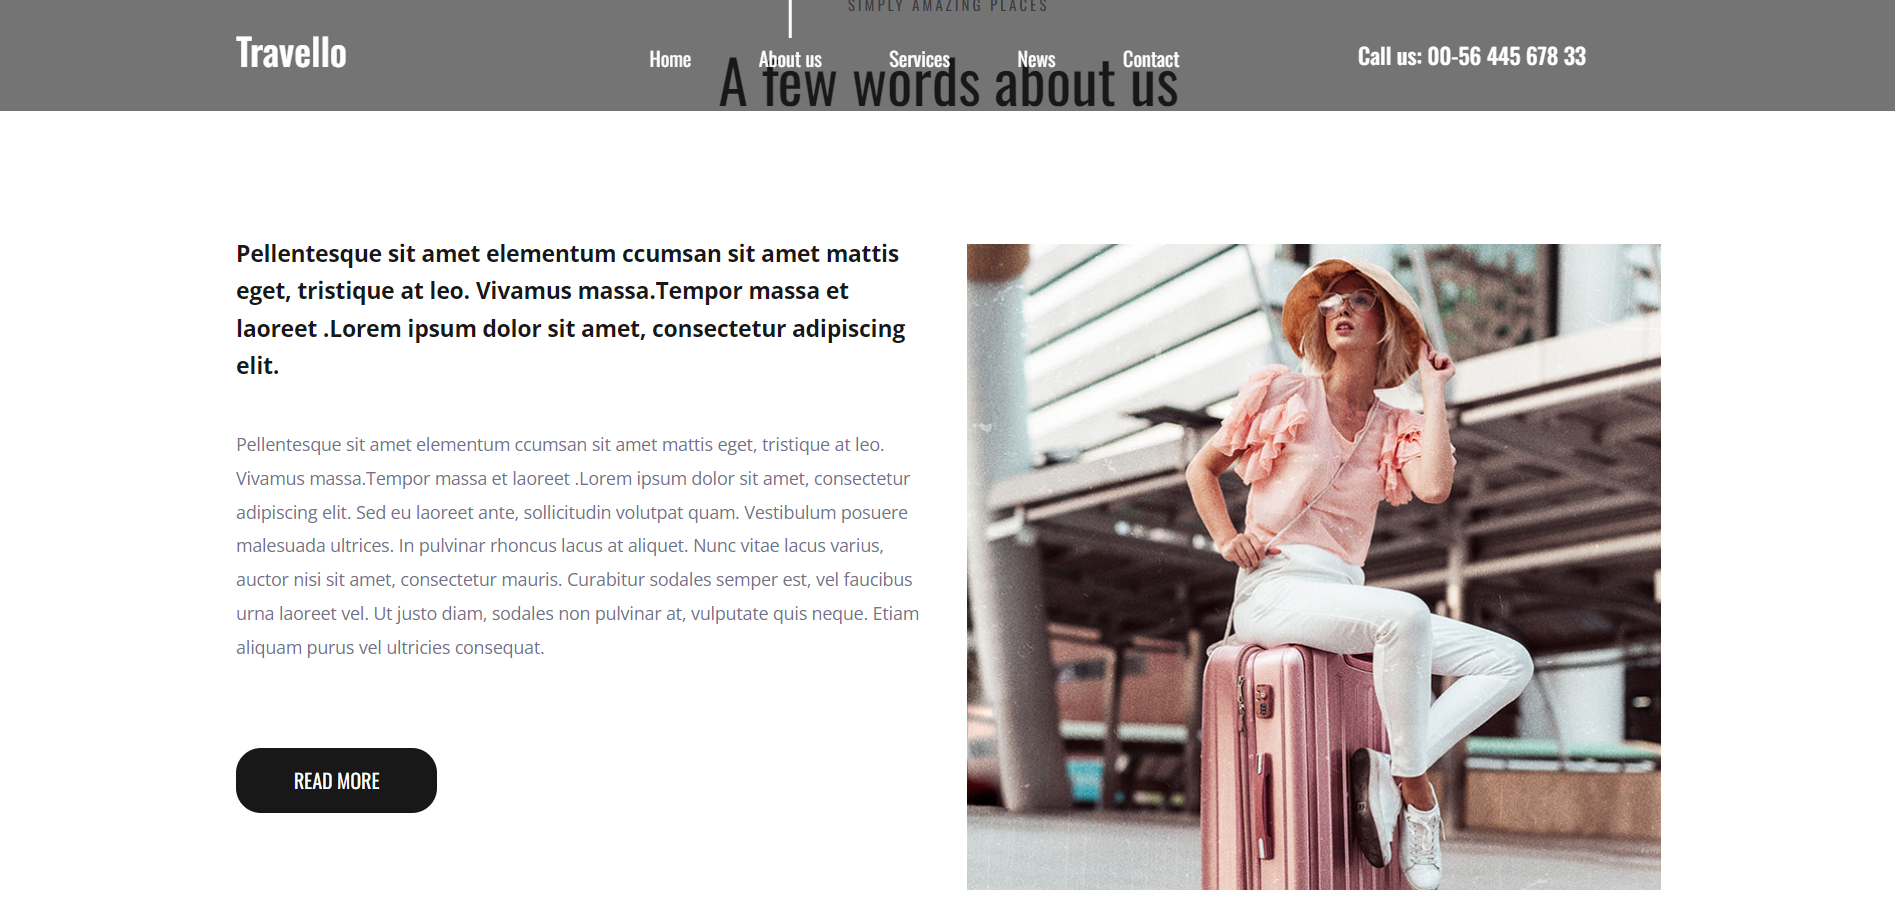
\includegraphics[width=1\textwidth, keepaspectratio]{img/ejecucion3.png}
    \caption{About}
  \end{figure}
  \newpage
  \begin{figure}[H]
    \centering
    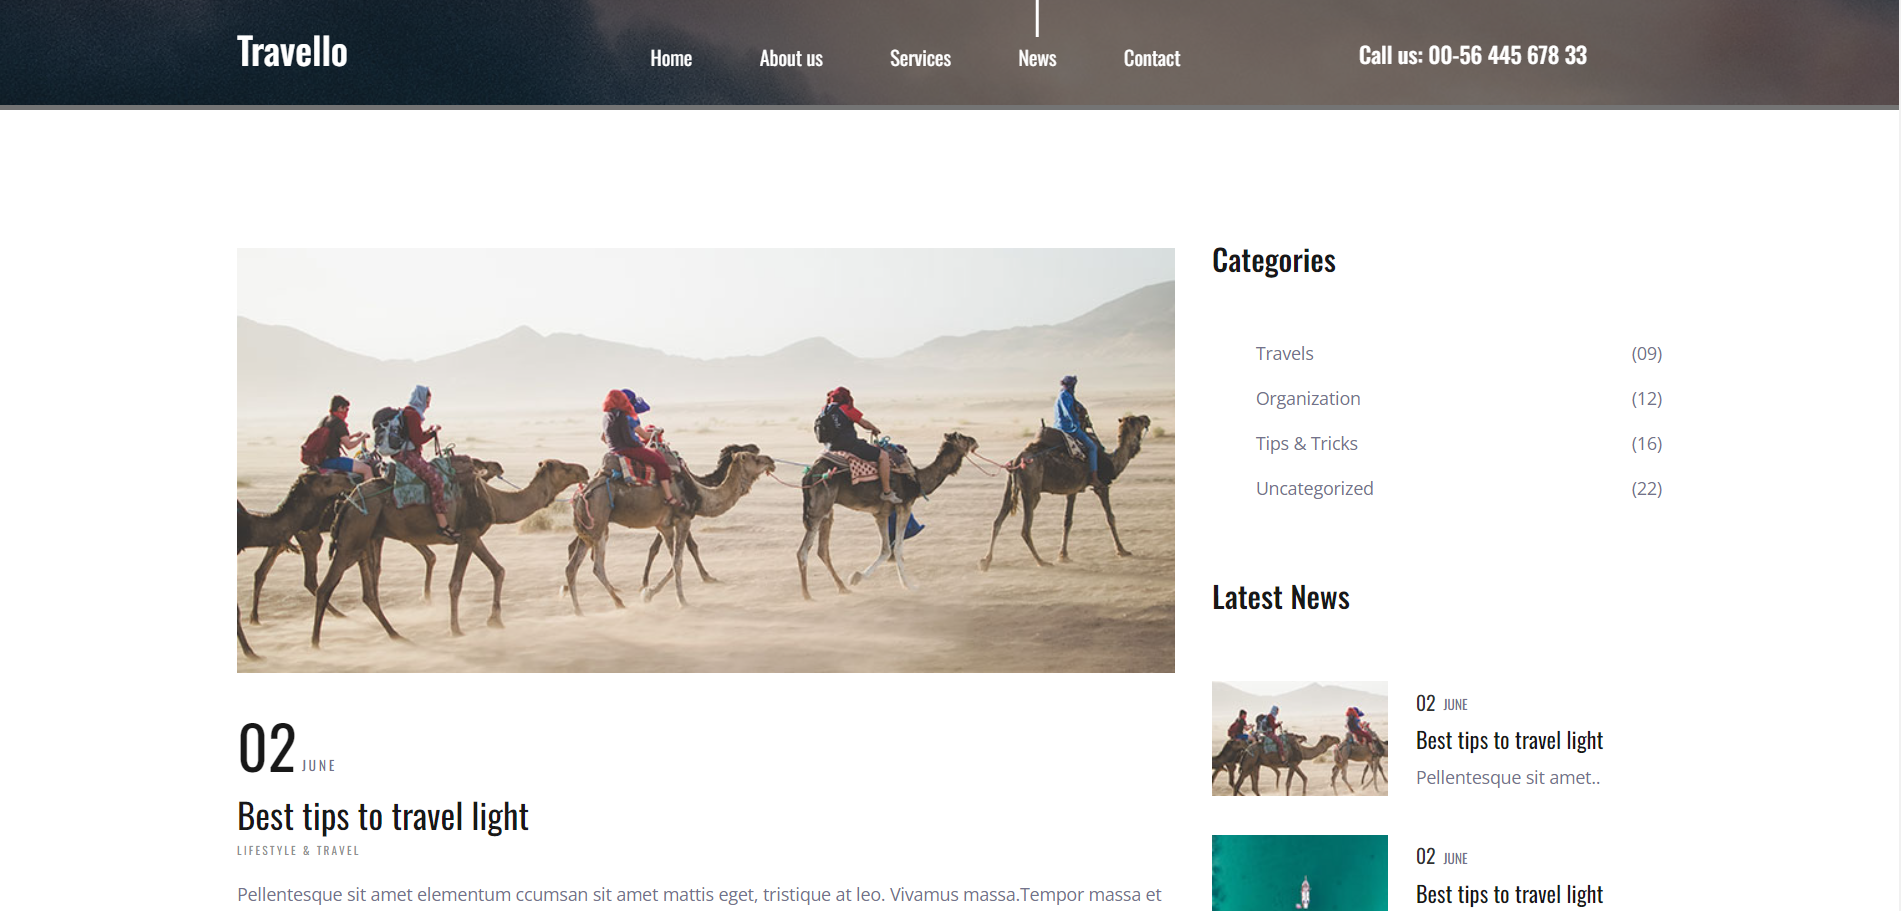
\includegraphics[width=1\textwidth, keepaspectratio]{img/ejecucion4.png}
    \caption{News}
  \end{figure}
  \begin{figure}[H]
    \centering
    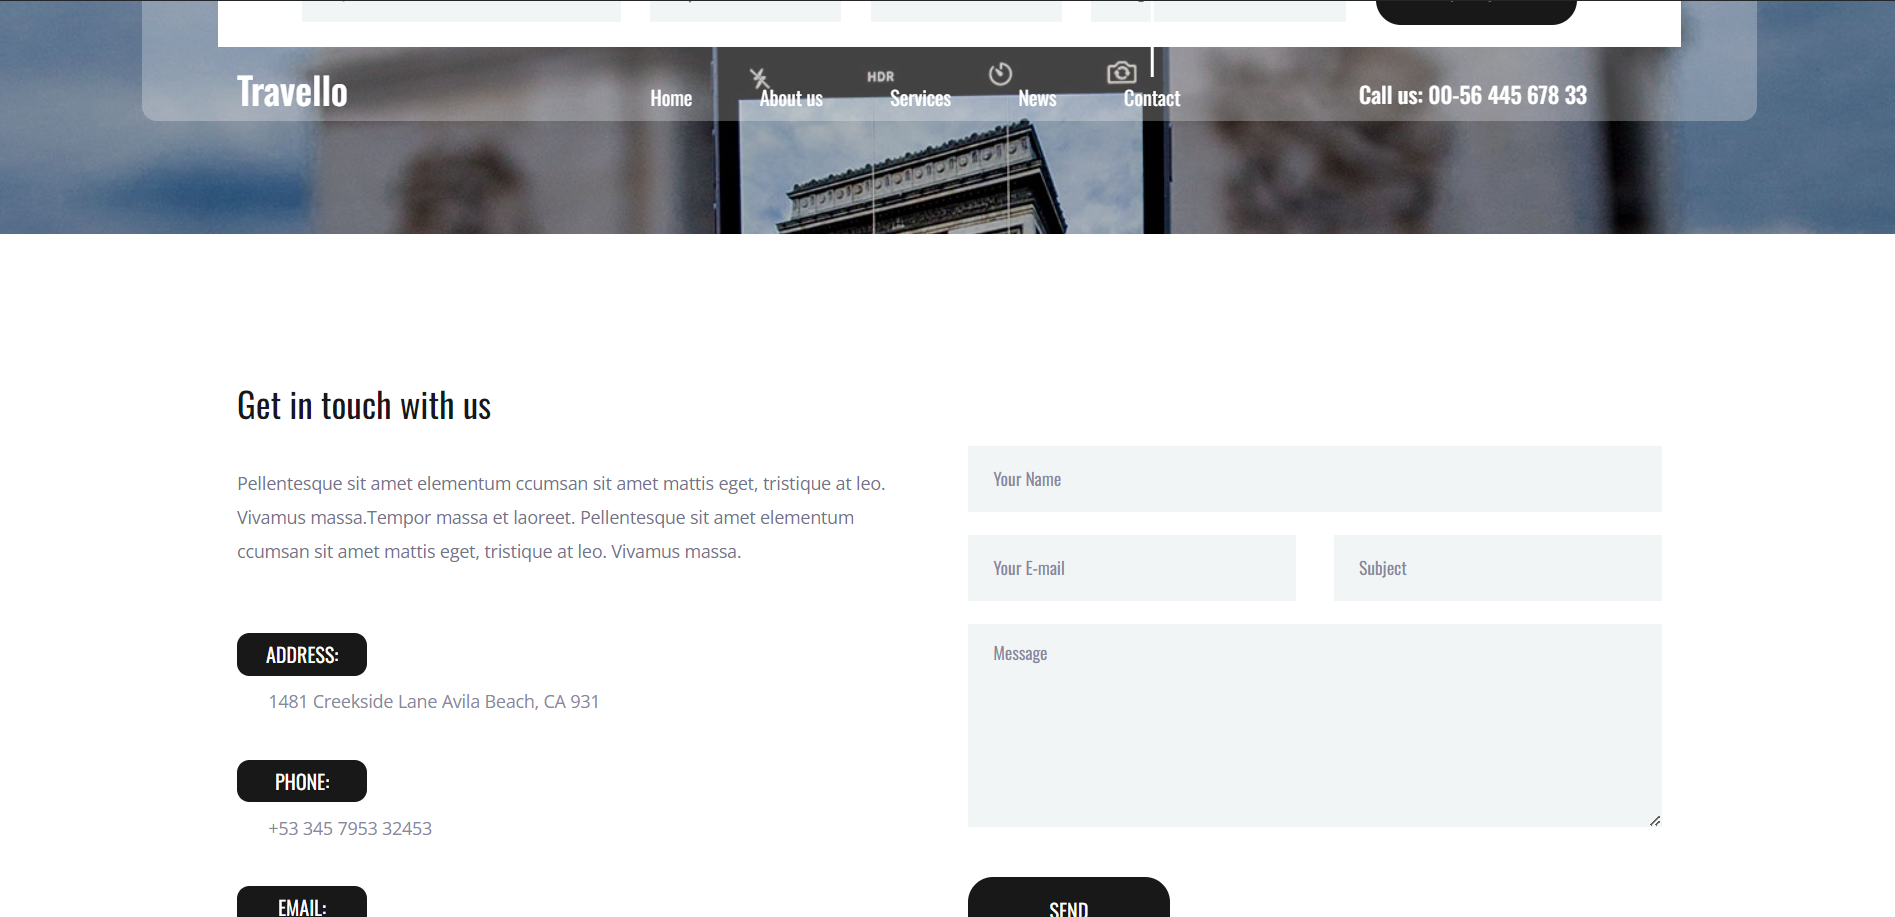
\includegraphics[width=1\textwidth, keepaspectratio]{img/ejecucion5.png}
    \caption{Contact}
  \end{figure}
  \newpage
  \begin{figure}[H]
    \centering
    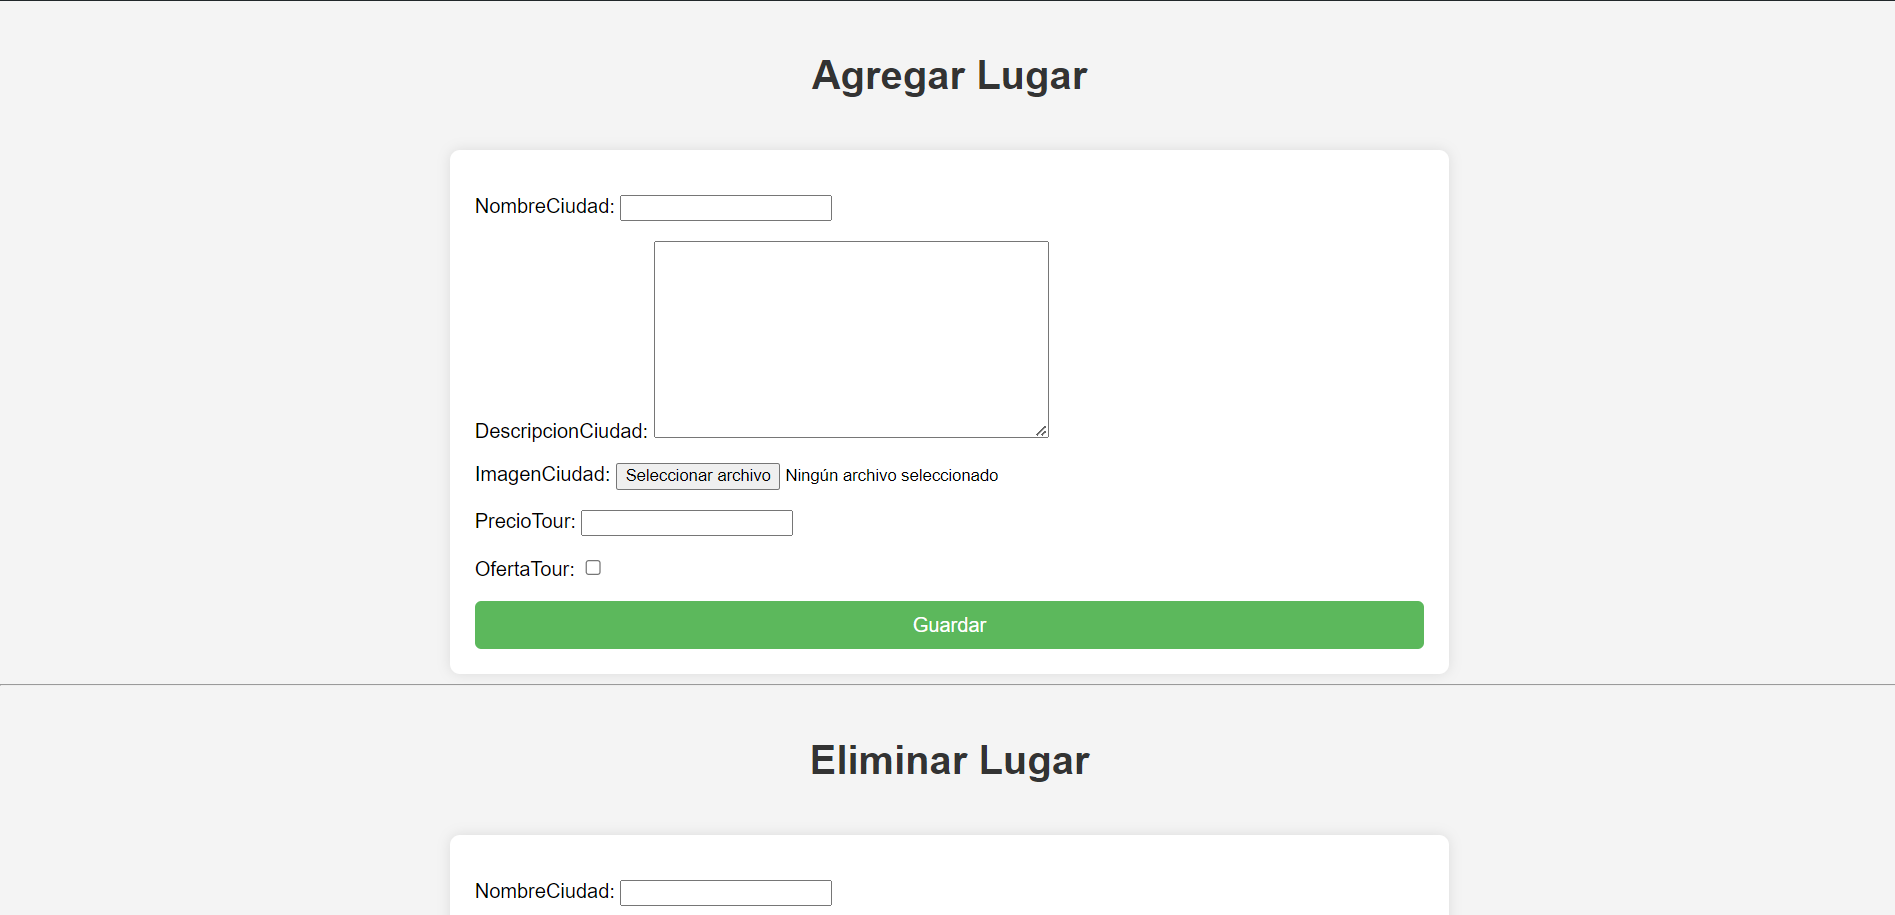
\includegraphics[width=1\textwidth, keepaspectratio]{img/ejecucion6.png}
    \caption{Admin - Formulario Agregar}
  \end{figure}
  \begin{figure}[H]
    \centering
    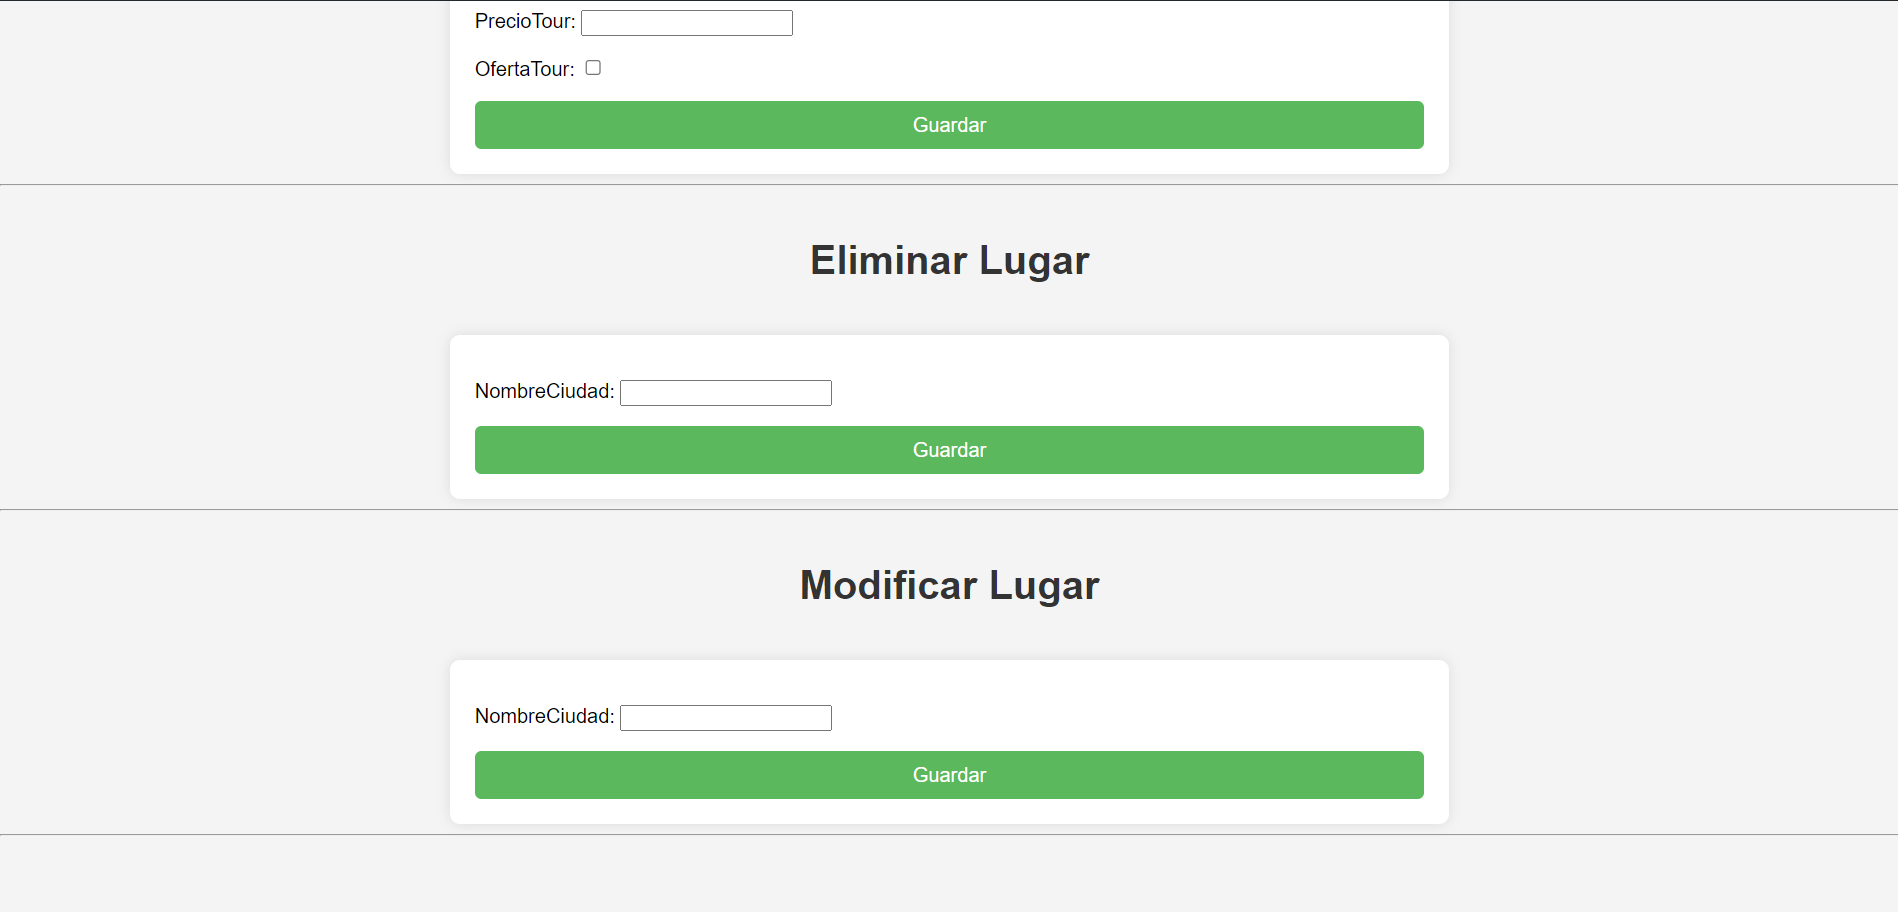
\includegraphics[width=1\textwidth, keepaspectratio]{img/ejecucion7.png}
    \caption{Admin - Formulario Eliminar y Modificar}
  \end{figure}
  \newpage
  \begin{figure}[H]
    \centering
    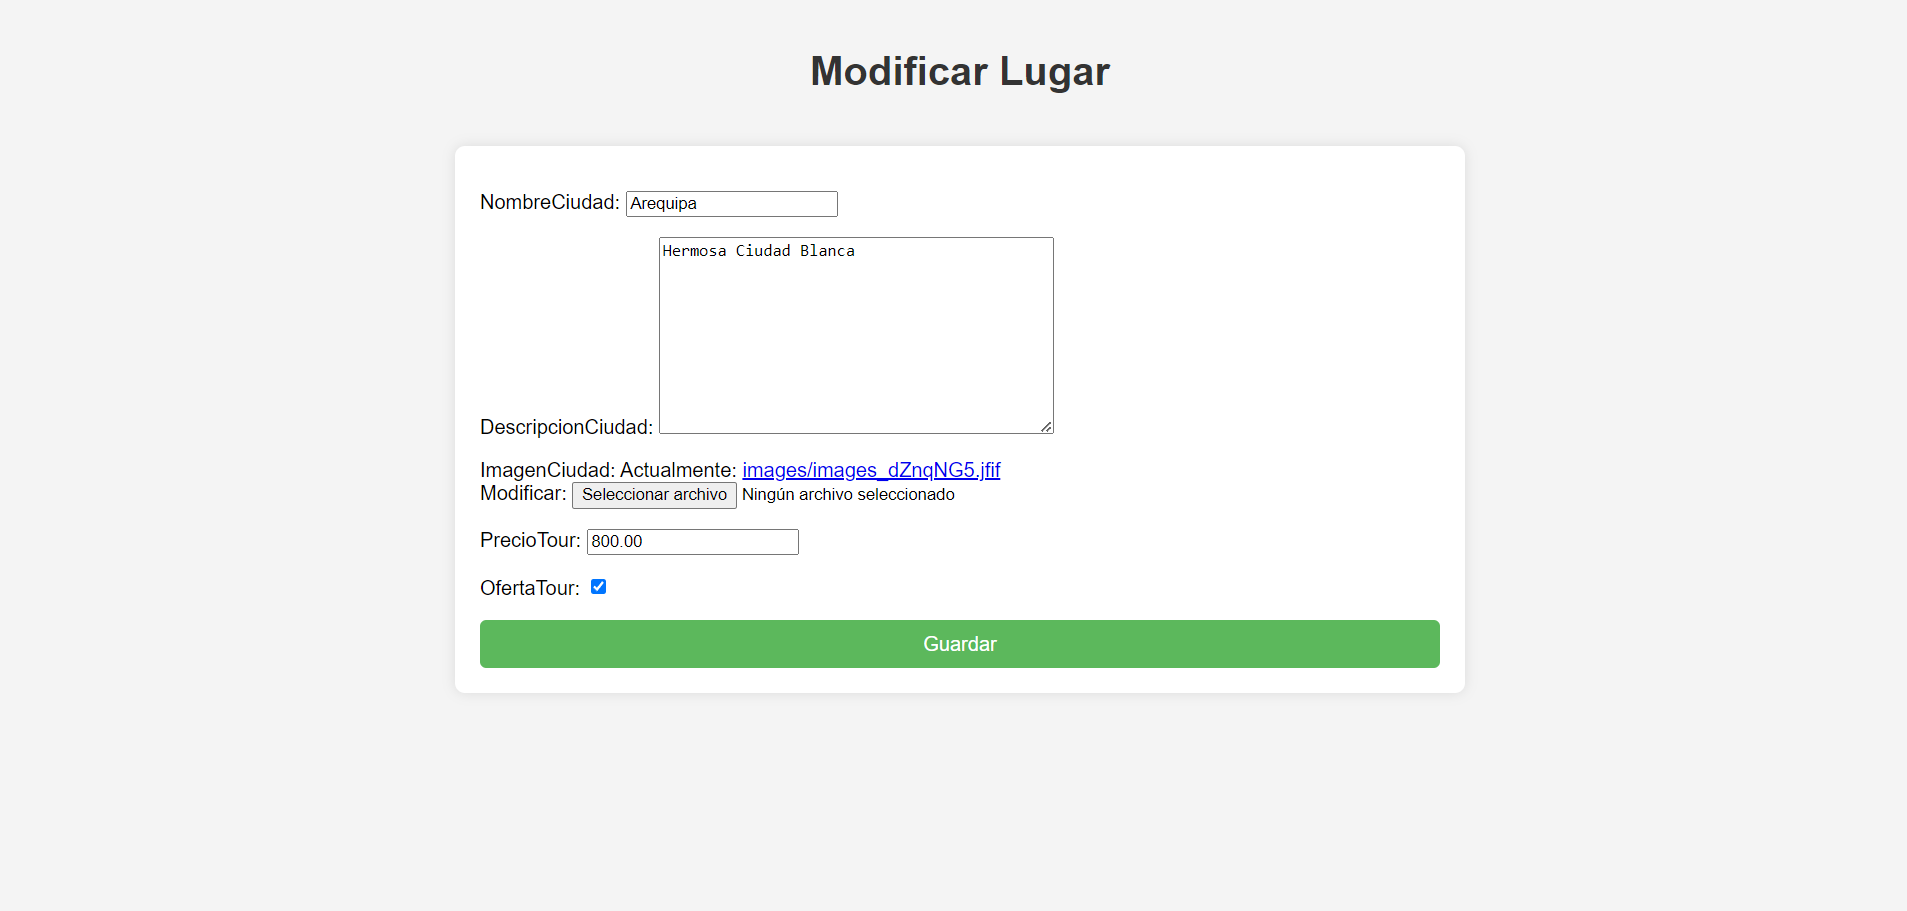
\includegraphics[width=1\textwidth, keepaspectratio]{img/ejecucion10.png}
    \caption{Admin - Formulario Modificar}
  \end{figure}
  \begin{figure}[H]
    \centering
    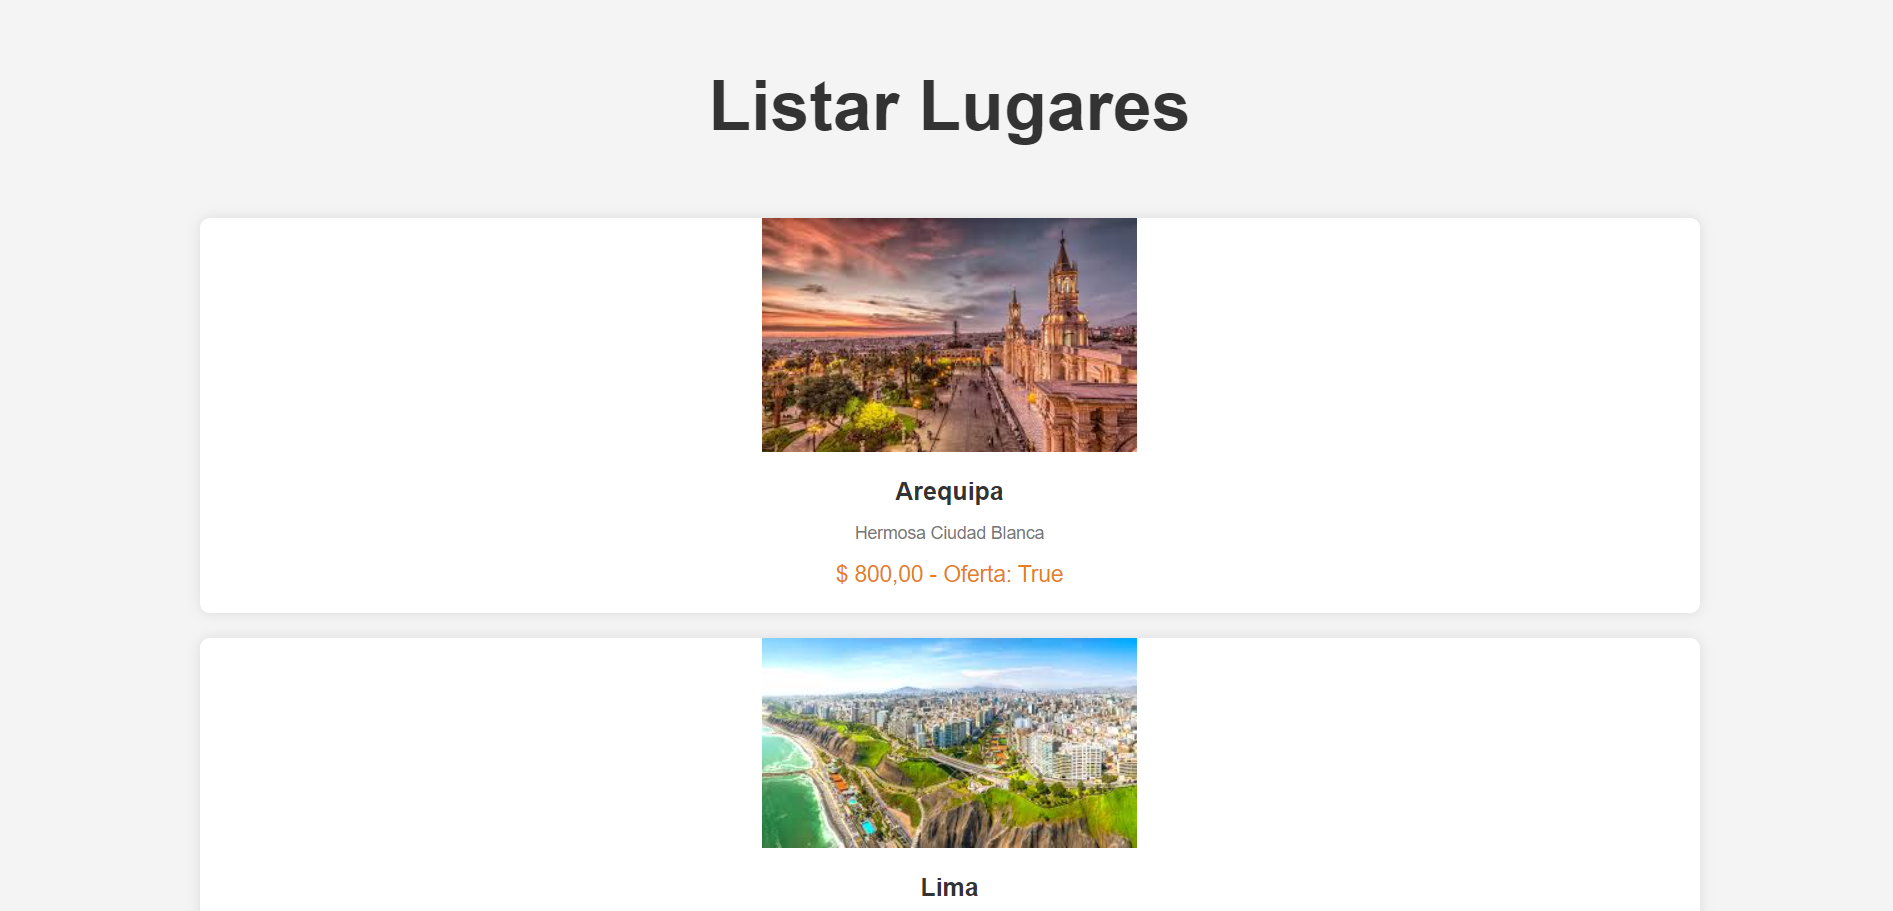
\includegraphics[width=1\textwidth, keepaspectratio]{img/ejecucion8.png}
    \caption{Admin - Listar 1}
  \end{figure}
  \newpage
  \begin{figure}[H]
    \centering
    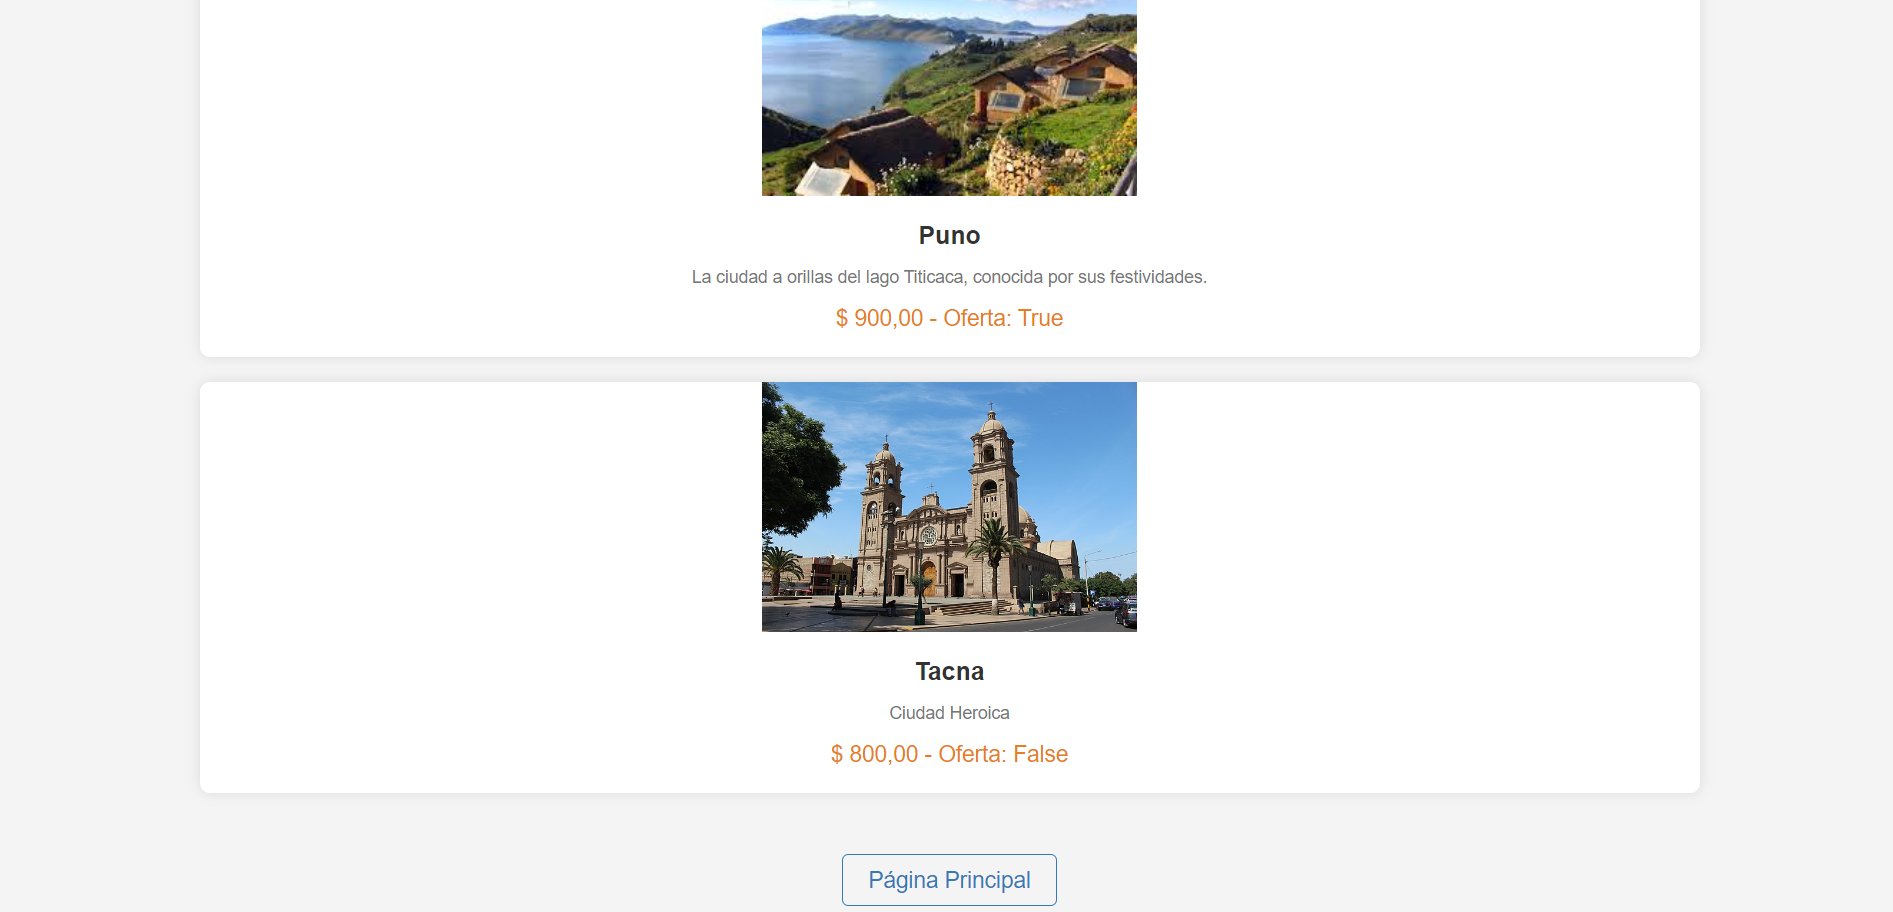
\includegraphics[width=1\textwidth, keepaspectratio]{img/ejecucion9.png}
    \caption{Admin - Listar 2}
  \end{figure}
  
%%%%%%%%%%%%%%%%%%%%
	
  \subsection{Uso de GitHub}
  
%%%%%%%%%%%%%%%%%%%%

	\subsubsection{Usuario de GitHub}
  \begin{figure}[H]
    \centering
    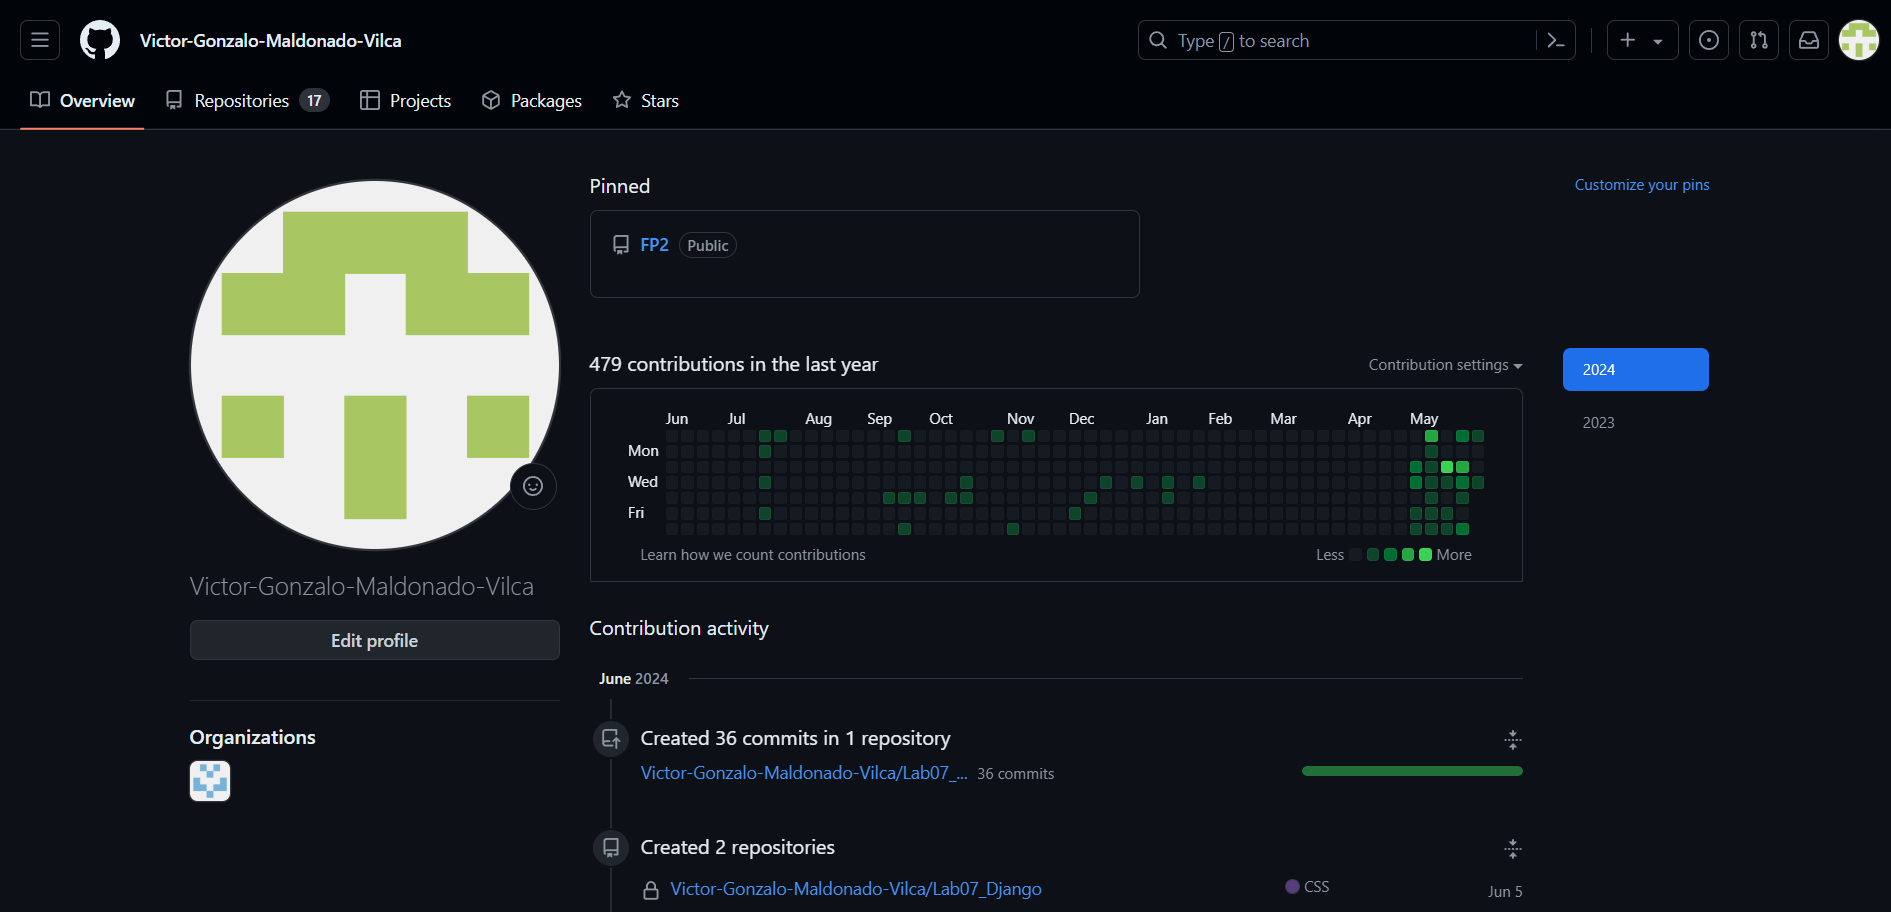
\includegraphics[width=1\textwidth, keepaspectratio]{img/usuario.png}
    \caption{Usuario}
  \end{figure}
  \newpage
  
%%%%%%%%%%%%%%%%%%%%

  \subsubsection{Creación de un Nuevo Repositorio}
  \begin{figure}[H]
    \centering
    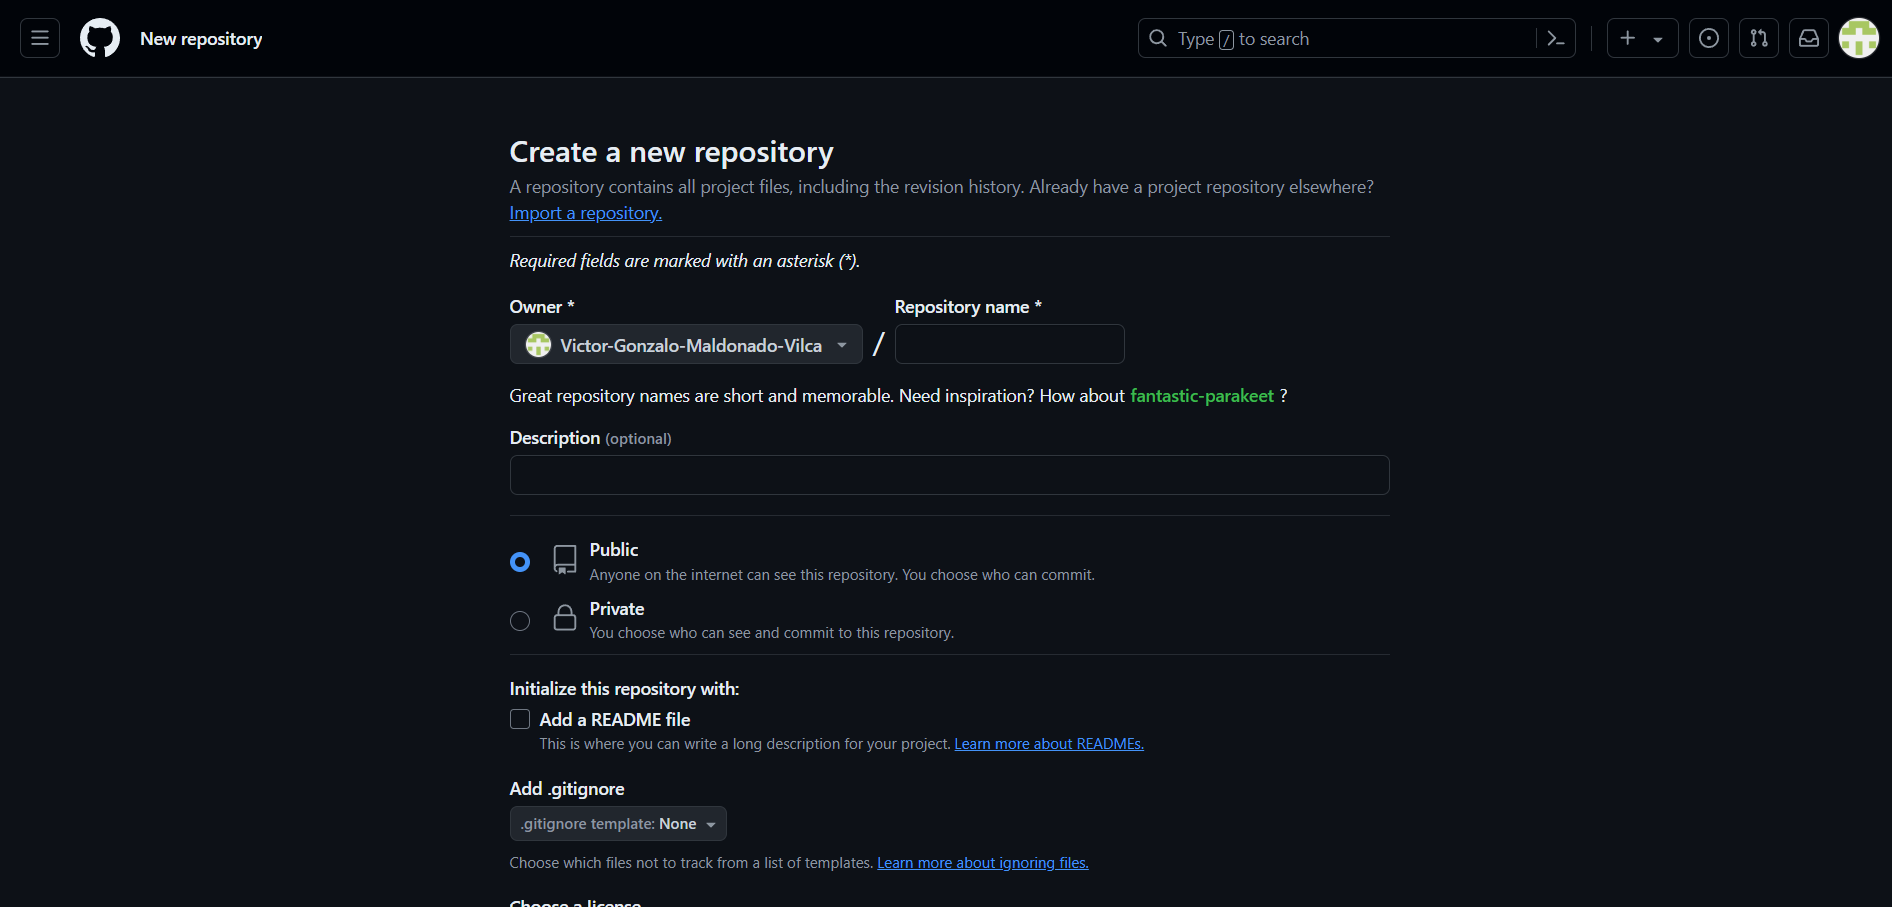
\includegraphics[width=1\textwidth, keepaspectratio]{img/crear.png}
    \caption{Nuevo Repositorio}
  \end{figure}
  
%%%%%%%%%%%%%%%%%%%%
	
  \subsubsection{Comandos de Configuración}
  \begin{lstlisting}[language=]
  echo "# lab07_Django" >> README.md
  git init
  git add README.md
  git commit -m "first commit"
  git branch -M master
  git remote add origin https://github.com/Victor-Gonzalo-Maldonado-Vilca/Lab07_Django.git
  git push -u origin master
  \end{lstlisting}
  \newpage
  
%%%%%%%%%%%%%%%%%%%%  
  
  \subsubsection{Implementación de Readme.md}
  \begin{figure}[H]
    \centering
    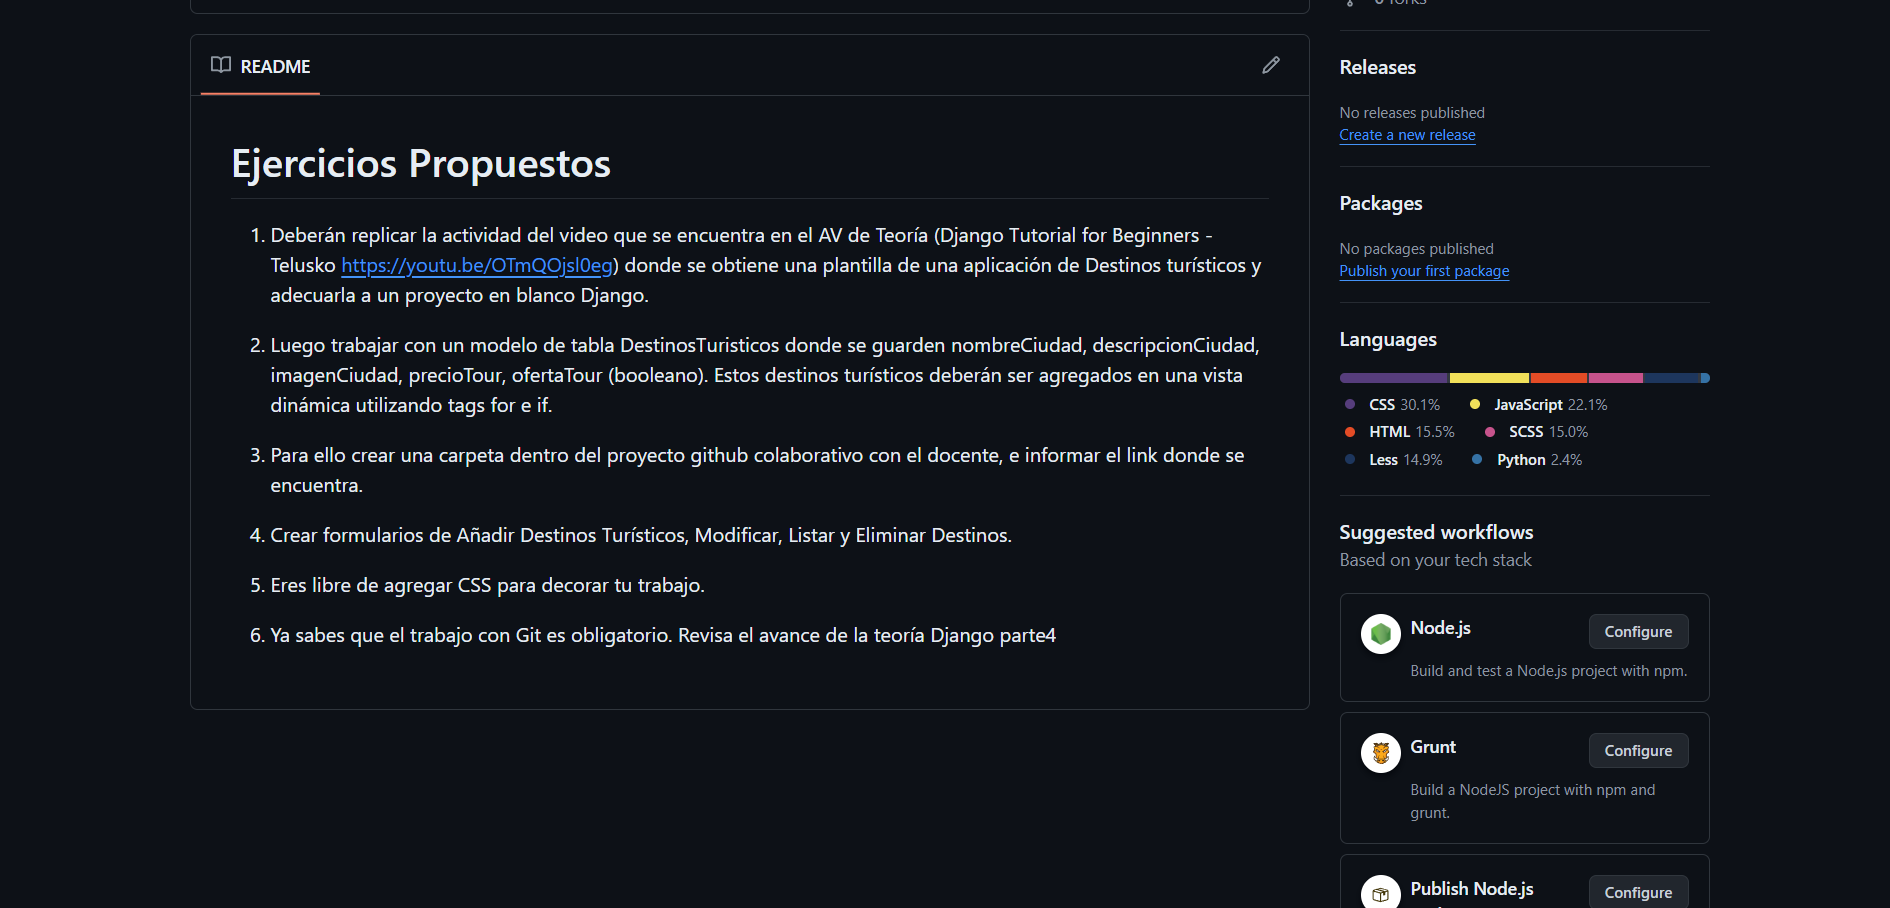
\includegraphics[width=1\textwidth, keepaspectratio]{img/readme.png}
    \caption{README.md}
  \end{figure}
  
%%%%%%%%%%%%%%%%%%%%

	\subsubsection{Registro de cambios en mi código}
  \begin{figure}[H]
    \centering
    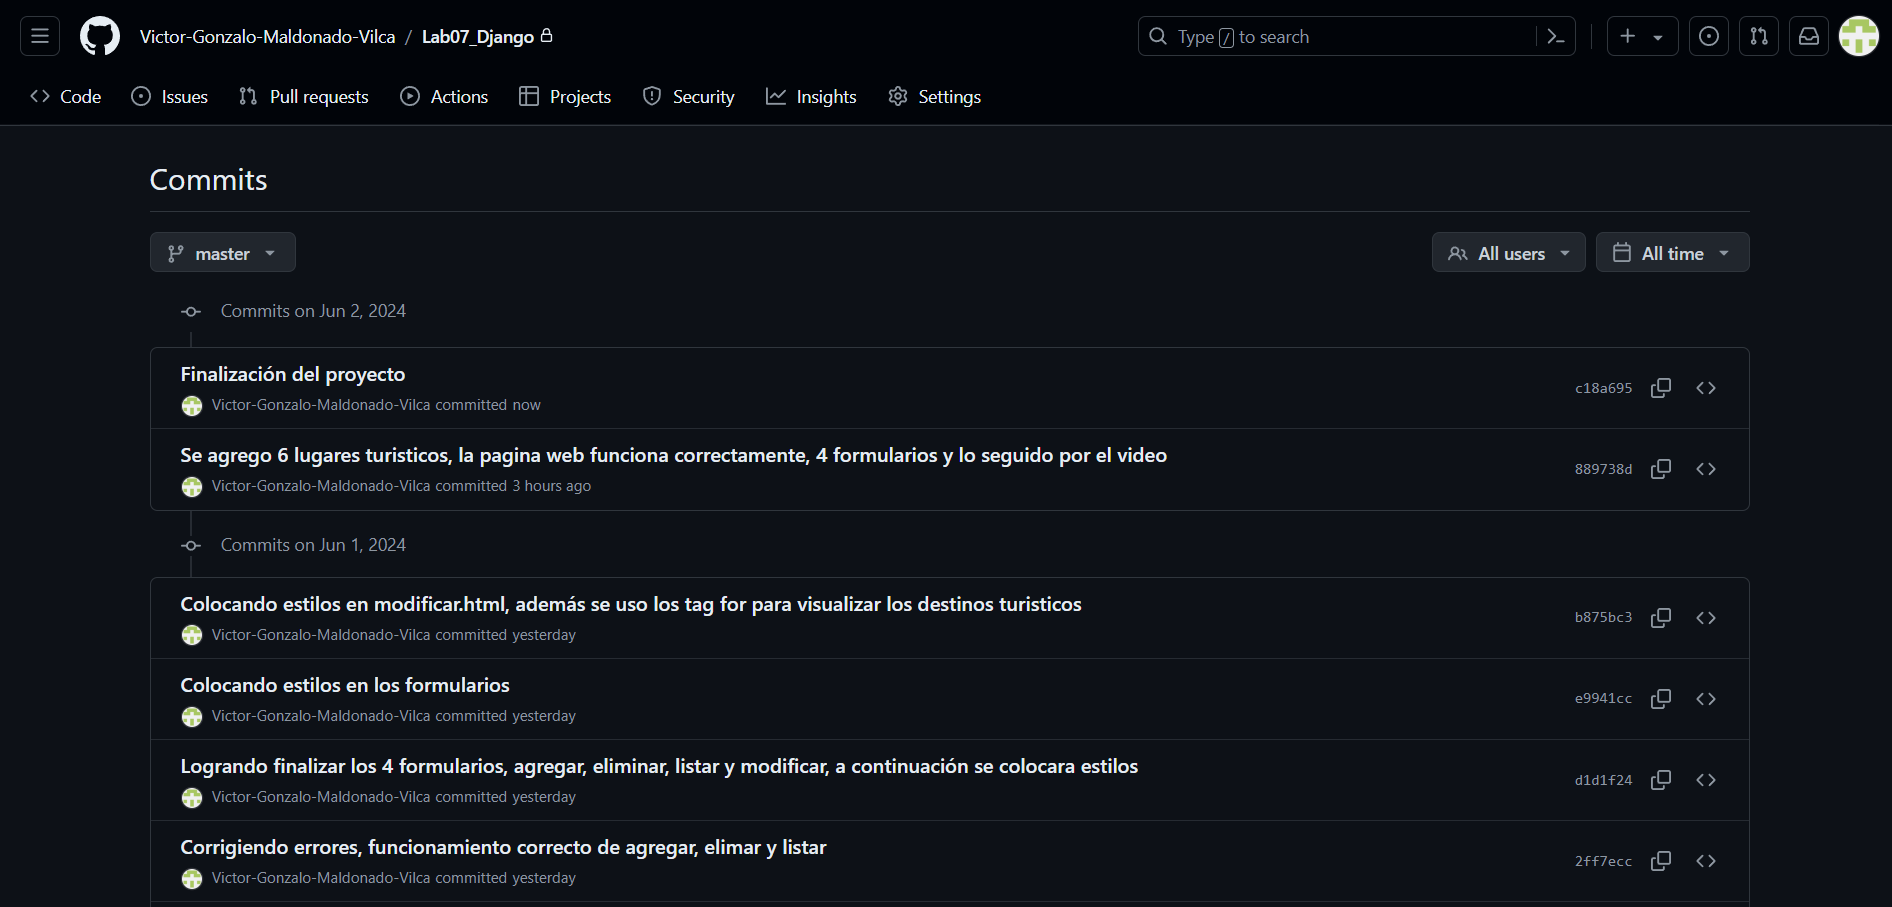
\includegraphics[width=1\textwidth, keepaspectratio]{img/commits.png}
    \caption{Commits}
  \end{figure}
  \newpage
	
%%%%%%%%%%%%%%%%%%%%

	\subsubsection{Repositorio}
  \begin{figure}[H]
    \centering
    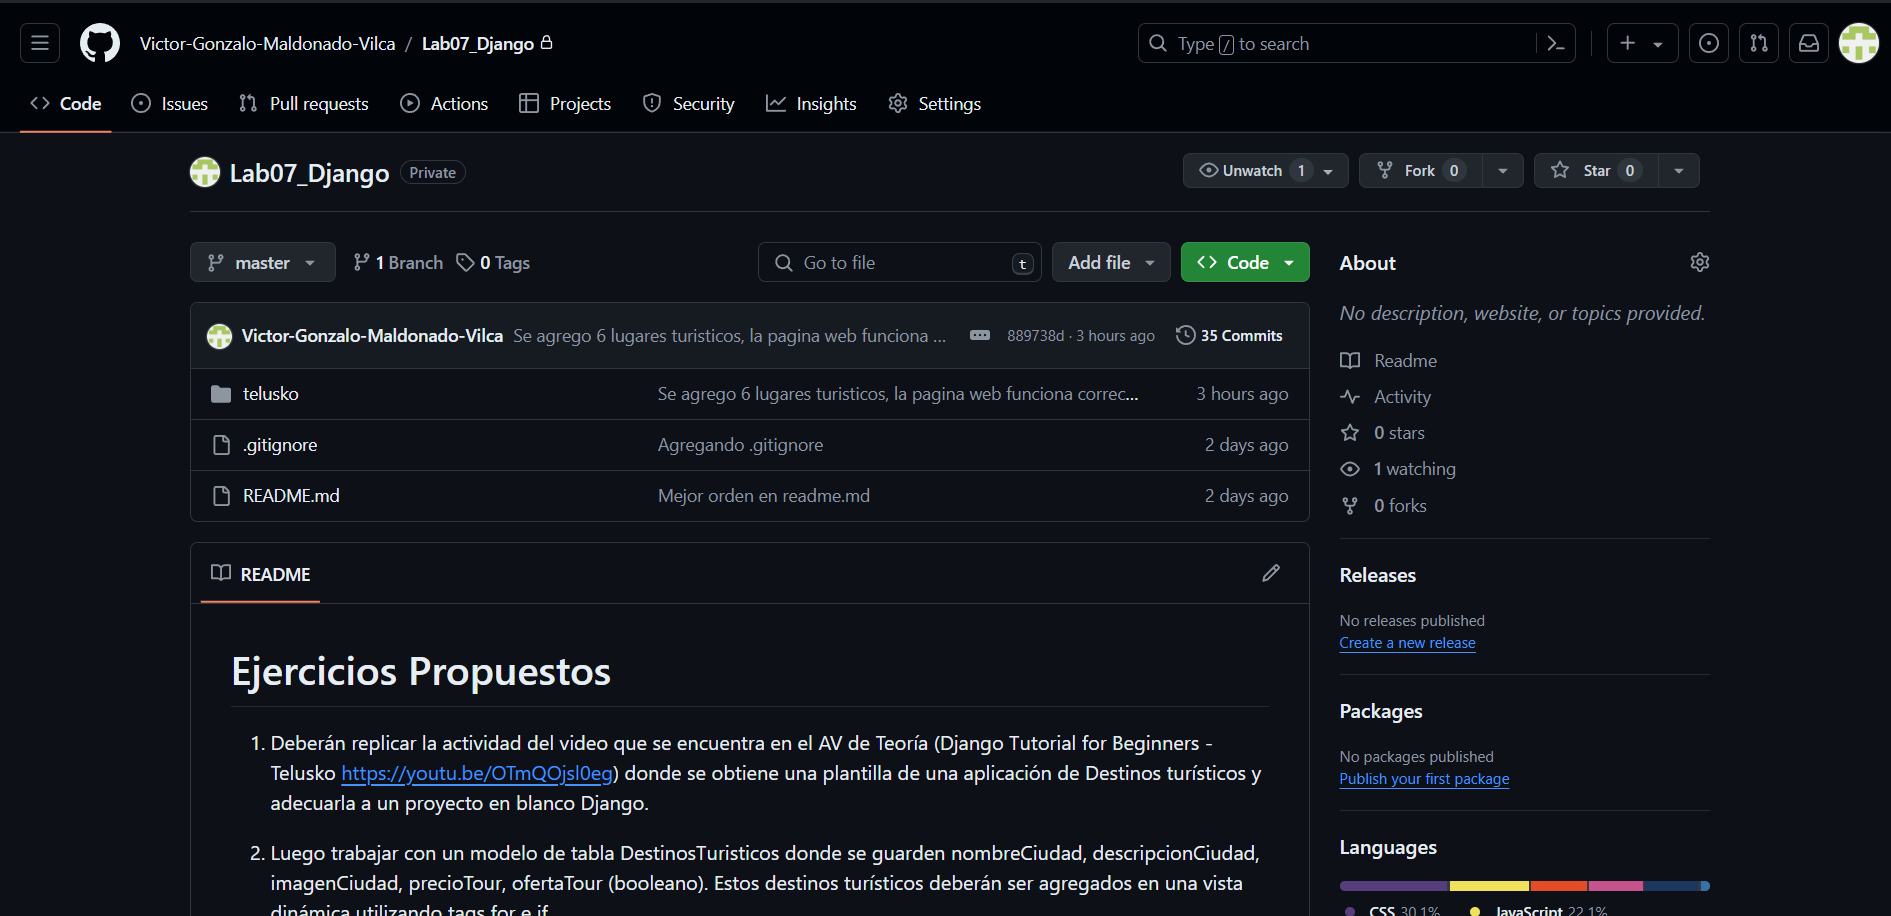
\includegraphics[width=1\textwidth, keepaspectratio]{img/repositorio.png}
    \caption{Repositorio}
  \end{figure}
  
%%%%%%%%%%%%%%%%%%%%

	\subsubsection{Proyecto compartido con el profesor de github}
  \begin{figure}[H]
    \centering
    \includegraphics[width=1\textwidth, keepaspectratio]{img/Compartir.png}
    \caption{Compartir con el Docente}
  \end{figure}
  \newpage
  
%%%%%%%%%%%%%%%%%%%%

  \section{Recomensaciones}
  \begin{itemize}
  \item Seguir las mejores prácticas de desarrollo de Django, como la separación de la lógica de negocios en vistas y 
  la creación de plantillas reutilizables.
  \item Realizar pruebas unitarias y de integración para garantizar la calidad del código, y asegúrate de implementar 
  medidas de seguridad en tu aplicación.
  \item Utilizar el sistema de plantillas de Django de manera efectiva para crear interfaces de usuario atractivas y funcionales.
  \item Implementar estrategias de caché y optimización de consultas para mejorar el rendimiento de la aplicación y reducir los tiempos de carga.
  \end{itemize}

%%%%%%%%%%%%%%%%%%%%

  \section{Conclusiones}
  \begin{itemize}
  \item Django es un framework web potente y versátil que permite desarrollar aplicaciones web de manera rápida y eficiente.
  \item La arquitectura MVC (Modelo-Vista-Controlador) de Django ayuda a organizar el código de manera estructurada y modular, 
    lo que facilita la mantenibilidad y escalabilidad de las aplicaciones.
  \item Con un buen entendimiento de Django y siguiendo las mejores prácticas de desarrollo, se pueden crear aplicaciones web 
    robustas y de alto rendimiento.
  \item Django proporciona una amplia gama de funcionalidades integradas, como autenticación de usuarios, administración de contenido 
  y seguridad, que facilitan el desarrollo de aplicaciones completas y seguras.
  \item La documentación detallada y los recursos de aprendizaje disponibles hacen que sea relativamente fácil para los desarrolladores aprender y dominar Django, lo que acelera el proceso de desarrollo y reduce los errores.
  \end{itemize}

%%%%%%%%%%%%%%%%%%%%
	\newpage
	\subsection{\textcolor{red}{Rúbrica para el contenido del Informe y demostración}}
	\begin{itemize}			
		\item El alumno debe marcar o dejar en blanco en celdas de la columna \textbf{Checklist} si cumplio con el ítem correspondiente.
		\item Si un alumno supera la fecha de entrega,  su calificación será sobre la nota mínima aprobada, siempre y cuando cumpla con todos lo items.
		\item El alumno debe autocalificarse en la columna \textbf{Estudiante} de acuerdo a la siguiente tabla:
	
		\begin{table}[ht]
			\caption{Niveles de desempeño}
			\begin{center}
			\begin{tabular}{ccccc}
    			\hline
    			 & \multicolumn{4}{c}{Nivel}\\
    			\cline{1-5}
    			\textbf{Puntos} & Insatisfactorio 25\%& En Proceso 50\% & Satisfactorio 75\% & Sobresaliente 100\%\\
    			\textbf{2.0}&0.5&1.0&1.5&2.0\\
    			\textbf{4.0}&1.0&2.0&3.0&4.0\\
    		\hline
			\end{tabular}
		\end{center}
	\end{table}	
	

	\end{itemize}

 
	
	\begin{table}[H]
		\caption{Rúbrica para contenido del Informe y demostración}
		\setlength{\tabcolsep}{0.5em} % for the horizontal padding
		{\renewcommand{\arraystretch}{1.5}% for the vertical padding
		%\begin{center}
		\begin{tabular}{|p{2.7cm}|p{7cm}|x{1.3cm}|p{1.2cm}|p{1.5cm}|p{1.1cm}|}
			\hline
    		\multicolumn{2}{|c|}{Contenido y demostración} & Puntos & Checklist & Estudiante & Profesor\\
			\hline
			\textbf{1. GitHub} & Hay enlace URL activo del directorio para el  laboratorio hacia su repositorio GitHub con código fuente terminado y fácil de revisar. &2 &X &2 & \\ 
			\hline
			\textbf{2. Commits} &  Hay capturas de pantalla de los commits más importantes con sus explicaciones detalladas. (El profesor puede preguntar para refrendar calificación). &4 &X &4 & \\ 
			\hline 
			\textbf{3. Código fuente} &  Hay porciones de código fuente importantes con numeración y explicaciones detalladas de sus funciones. &2 &X &2 & \\ 
			\hline 
			\textbf{4. Ejecución} & Se incluyen ejecuciones/pruebas del código fuente  explicadas gradualmente. &2 &X &2 & \\ 
			\hline			
			\textbf{5. Pregunta} & Se responde con completitud a la pregunta formulada en la tarea.  (El profesor puede preguntar para refrendar calificación).  &2 &X &2 & \\ 
			\hline	
			\textbf{6. Fechas} & Las fechas de modificación del código fuente estan dentro de los plazos de fecha de entrega establecidos. &2 &X &2 & \\ 
			\hline 
			\textbf{7. Ortografía} & El documento no muestra errores ortográficos. &2 &X &2 & \\ 
			\hline 
			\textbf{8. Madurez} & El Informe muestra de manera general una evolución de la madurez del código fuente,  explicaciones puntuales pero precisas y un acabado impecable.   (El profesor puede preguntar para refrendar calificación).  &4 &X &4 & \\ 
			\hline
			\multicolumn{2}{|c|}{\textbf{Total}} &20 & &20 & \\ 
			\hline
		\end{tabular}
		%\end{center}
		%\label{tab:multicol}
		}
	\end{table}


%%%%%%%%%%%%%%%%%%%%%%%%%%%%%%%%%%%%%%%%%%%%%%%%%%%%%%%%%%%%%%%%%%%
	
  \newpage
  \section{Referencias}
  \begin{itemize}
    \item \url{https://docs.djangoproject.com/en/5.0/}
    \item \url{https://docs.github.com/es}
    \item \url{https://git-scm.com/doc}
    \item \url{https://www.youtube.com/watch?v=OTmQOjsl0eg}
    \item \url{https://www.dropbox.com/sh/gf8x8xjwidq20cz/AABPlOsXmijnz0-yjxYj9ebsa?dl=0}
  \end{itemize}

%%%%%%%%%%%%%%%%%%%% 
%\clearpage
%\bibliographystyle{apalike}
%\bibliographystyle{IEEEtranN}
%\bibliography{bibliography}
			
\end{document}
